%% 美赛模板:正文部分

\documentclass[12pt]{article}  % 官方要求字号不小于 12 号,此处选择 12 号字体
% 本模板不需要填写年份,以当前电脑时间自动生成
% 请在以下的方括号中填写队伍控制号
\usepackage[2321846]{easymcm}  % 载入 EasyMCM 模板文件
\problem{C}  % 请在此处填写题号
 \usepackage{mathptmx}  % 这是 Times 字体,中规中矩 
%\usepackage{mathpazo}  % 这是 COMAP 官方杂志采用的更好看的 Palatino 字体,可替代以上的 mathptmx 宏包
\title{WORDLE Play, WORDLE Study}  % 标题
\usepackage{enumerate}
\usepackage{lettrine}
\usepackage[ruled,linesnumbered]{algorithm2e}
\usepackage{lipsum}
\usepackage{hyperref}
\usepackage{adjustbox}
% 如需要修改题头(默认为 MCM/ICM),请使用以下命令(此处修改为 MCM)
%\renewcommand{\contest}{MCM}
\usepackage{bm}
\usepackage{cleveref}
\usepackage{ulem}
\usepackage{geometry}
\usepackage{framed} 
\usepackage{mathrsfs}
\usepackage{lettrine}
\usepackage{wasysym}
\usepackage[table,xcdraw]{xcolor}
 \usepackage{booktabs}
 \usepackage{multirow}
 \usepackage{makecell}
% \usepackage[table,xcdraw]{xcolor}
% If you use beamer only pass "xcolor=table" option, i.e. \documentclass[xcolor=table]{beamer}
 % \usepackage[normalem]{ulem}



\begin{document}

% 此处填写摘要内容
\begin{abstract}
``WORDLE'', a popular game that went viral on Twitter as soon as it was introduced. It has very simple rules: you just need to rely on your vocabulary and reasoning skills using no more than 6 chances to guess the word of that day. Now we've been invited by the New York Times to conduct the following research around it.

First, we built ARIMA model to predict the number of future reports and predicted the number of reports in the interval [30943,33839] on March 1, 2023 based on the model and the inherent error of the model. The accuracy of the model, which was trained and tested using an 8:2 ratio, was determined to be 84.46\%.

To further improve the accuracy, we used a temporal recurrent neural network---LSTM model, to improve the ARIMA model and built an LSTM-ARIMA model to predict the associated percentages of (1, 2, 3, 4, 5, 6, X) for a future date. without considering the effect of word difficulty on the model. The predicted percentages of (1, 21, 12, 14, 30, 18, 4) for the word ``EERIE'' on March 1, 2023 without considering the effect of word difficulty on the model, and the accuracy of the test set was calculated to be 93.37\% within 1\% error.

We applied the cubic equation to fit the percentage of scores reported that were played in Hard Mode, and obtained the cubic equation $y=8.841e^{-10}x^3-1.271e^{-6}x^2+0.0005522x+0.02044$ for the percentage of people playing in Hard Mode over time. The goodness of fit ($R^2$) was reaches 0.9681 (The closer $R^2$ is to 1, the better the fit is), so it is clear that as people become more proficient at the game over time, more and more people try the difficult mode. Since people did not know any properties of the word of the day until they chose the mode and successfully guessed the word, we infer that the percentage of scores reported that were played in Hard Mode did not vary with the properties of the words themselves.

And then we investigated the characteristics of the words themselves, we used multiple linear regression model to test the correlation of the factors we guessed might affect the difficulty of the words, and identified the main five main factors that affect the difficulty of the words in the game (Average number of words, Average score of lexical categories, Average number of non-repeating letters, Percentage of letter appearances, Average number of word meanings) as evaluation indexes. Established the AHP-EWM-TOPSIS model, the factor with the highest weight calculated by the entropy weighting method and the factor with the highest fit in the regression model are both ``Average number of word meanings''. Then, the words were classified into 5 levels of difficulty according to their scores: Entry, Intermediate, Advanced, Hard, and Hell. We used this model to calculate the difficulty level of ``EERIE'' as ``Hell Level''. We then defined the accuracy of the model and calculated an accuracy rate of 79.60\%.

In addition, we found some other interesting features, such as the fact that only a very small number of people in the data did not guess the words and a tip to improve the success rate.

Finally, we wrote a letter to the Puzzle Editor of the New York Times to summarize our results and put forward some suggestions for the future development of ``WORDLE''.

    \vspace{5pt}
    \textbf{Keywords}:WORDLE, ARIMA Model, LSTM-ARIMA Model, AHP-EWM-TOPSIS Model    

\end{abstract}

\maketitle 
 % 生成 Summary Sheet
\tableofcontents
% 正文开始
\section{Introduction}
\subsection{Background}
% \begin{figure}[htbp]
% \centering
% \includegraphics[width=\textwidth]{img/s.pdf}
% % \caption{Our Work}
% \end{figure}
What is ``WORDLE''? Let me tell you that ``WORDLE'' is a daily word game which wave has swept the world since January 2022, the articles about it have 197,000,000 results on Google search. And there are even more Twitters about it, and you can always receive feedback from different people about the game of the day.If you want to know more about this game, you can go to its official website and try it, we guarantee you will be fascinated by it.

Are there any other interesting reasons behind the seemingly untechnical and inexplicable word guessing game. Our team was interested in this and was invited by the New York Times to make the following analysis.
\subsection{Restatement and Analysis of Problems}
In this paper, we reordered the unordered list of topics in order to make the passage smoother. We divided the problems that needed to be solved into three tasks:
\begin{enumerate}
\renewcommand{\labelenumi}{{\sc Task} \theenumi}
\item Analyzing and fitting the data we obtained includes Number of reported results, Number in hard mode (reflected here in the paper where we processed it to get the percentage of games in hard mode), the proportion of different guesses. and using the model we built to predict how they will change in the future, giving a reasonable prediction of each data for March 1, 2023. We also use the model to explain the results of our predictions and the reasons for them under reasonable assumptions and analysis.
\item Find the effect of the properties of the words themselves on the difficulty of the wordle words, classify the difficulty of the words in the game and give the criteria and reasons for our classification, and find the common features of words with the same difficulty. Use our model to determine the difficulty of the word ``EERIE''.
\item This paper discusses the advantages and disadvantages of our model, analyzes the uncertainty and confidence of our model, and looks for the available information and some undiscovered information in the data set. Report our results to the Puzzle Editor of the New York Times.
\end{enumerate}
\subsection{Our Work}
{\LARGE\CheckedBox} ARIMA model and LSTM-ARIMA model are built to fit our data set and predict the number of people playing ``WORDLE'' on March 1, 2023 and the proportion of times of guessing words.

{\LARGE\CheckedBox} Find out the attributes of the word itself and establish the AHP-EWM-TOPSIS model to score the difficulty of the word and then get different difficulty levels. Use our model to judge the difficulty level of the word ``EERIE''.

{\LARGE\CheckedBox} We evaluated our model and found some other interesting features in the data set. Summarize our findings and share them with the Puzzle Editor of the New York
Times.
\begin{figure}[htbp]
\centering
\includegraphics[width=0.6\textwidth]{img/OURWORK.pdf}
\caption{Our Work}
\end{figure}
% \begin{figure}[htbp]
% \centering
% \includegraphics[width=\textwidth]{img/lstm.pdf}
% % \caption{Our Work}
% \end{figure}
% \begin{figure}[htbp]
% \centering
% 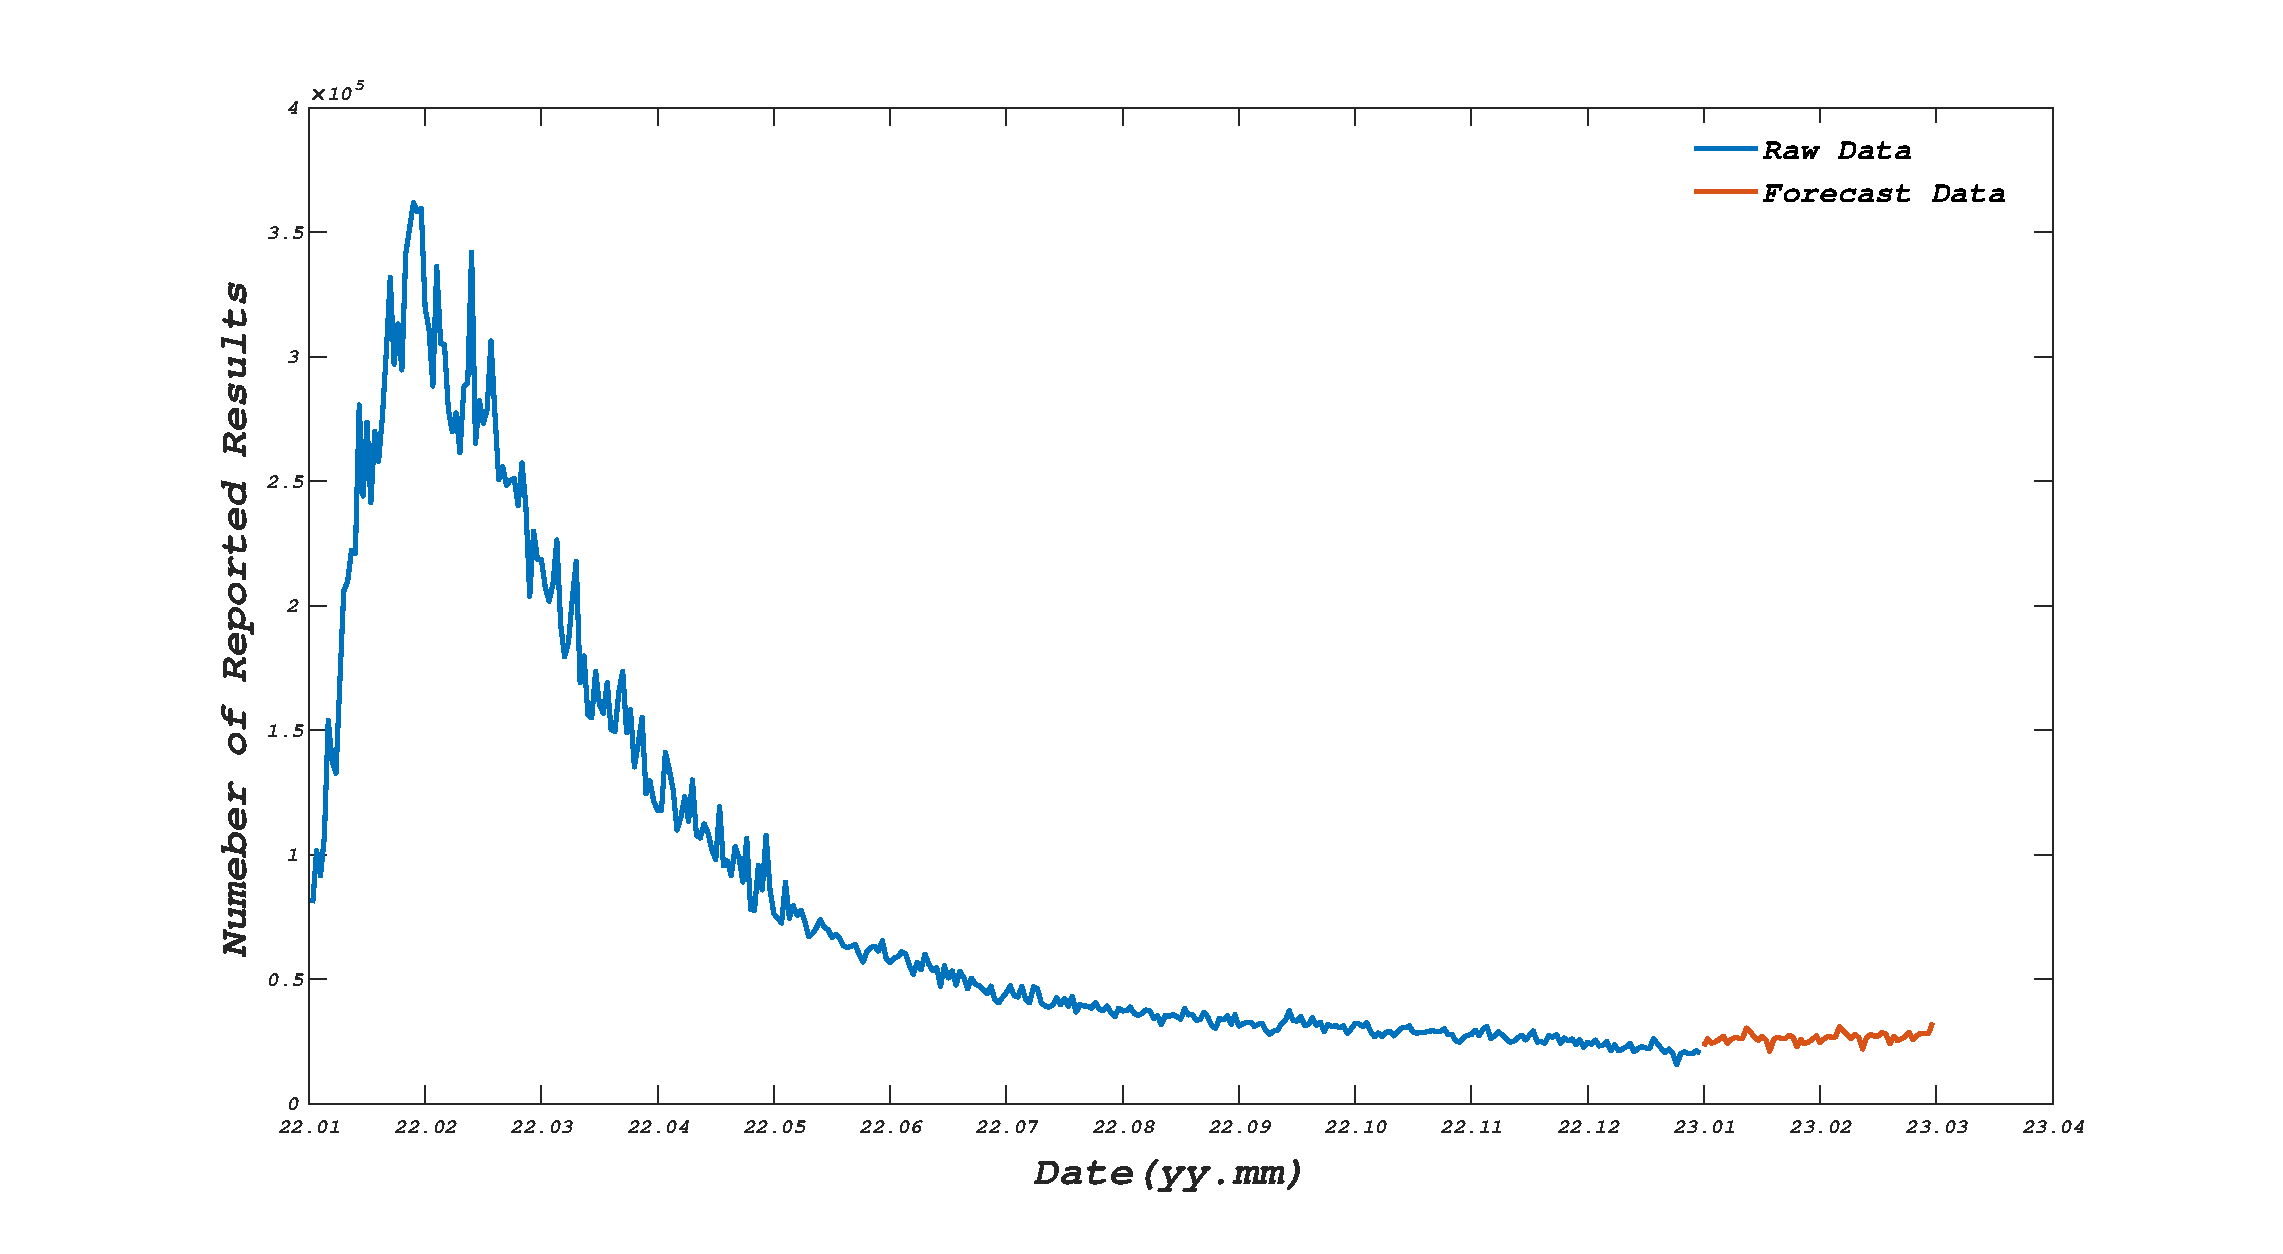
\includegraphics[width=\textwidth]{img/yuce.eps}
% \caption{forecast}
% \end{figure}
% \begin{figure}[htbp]
% \centering
% 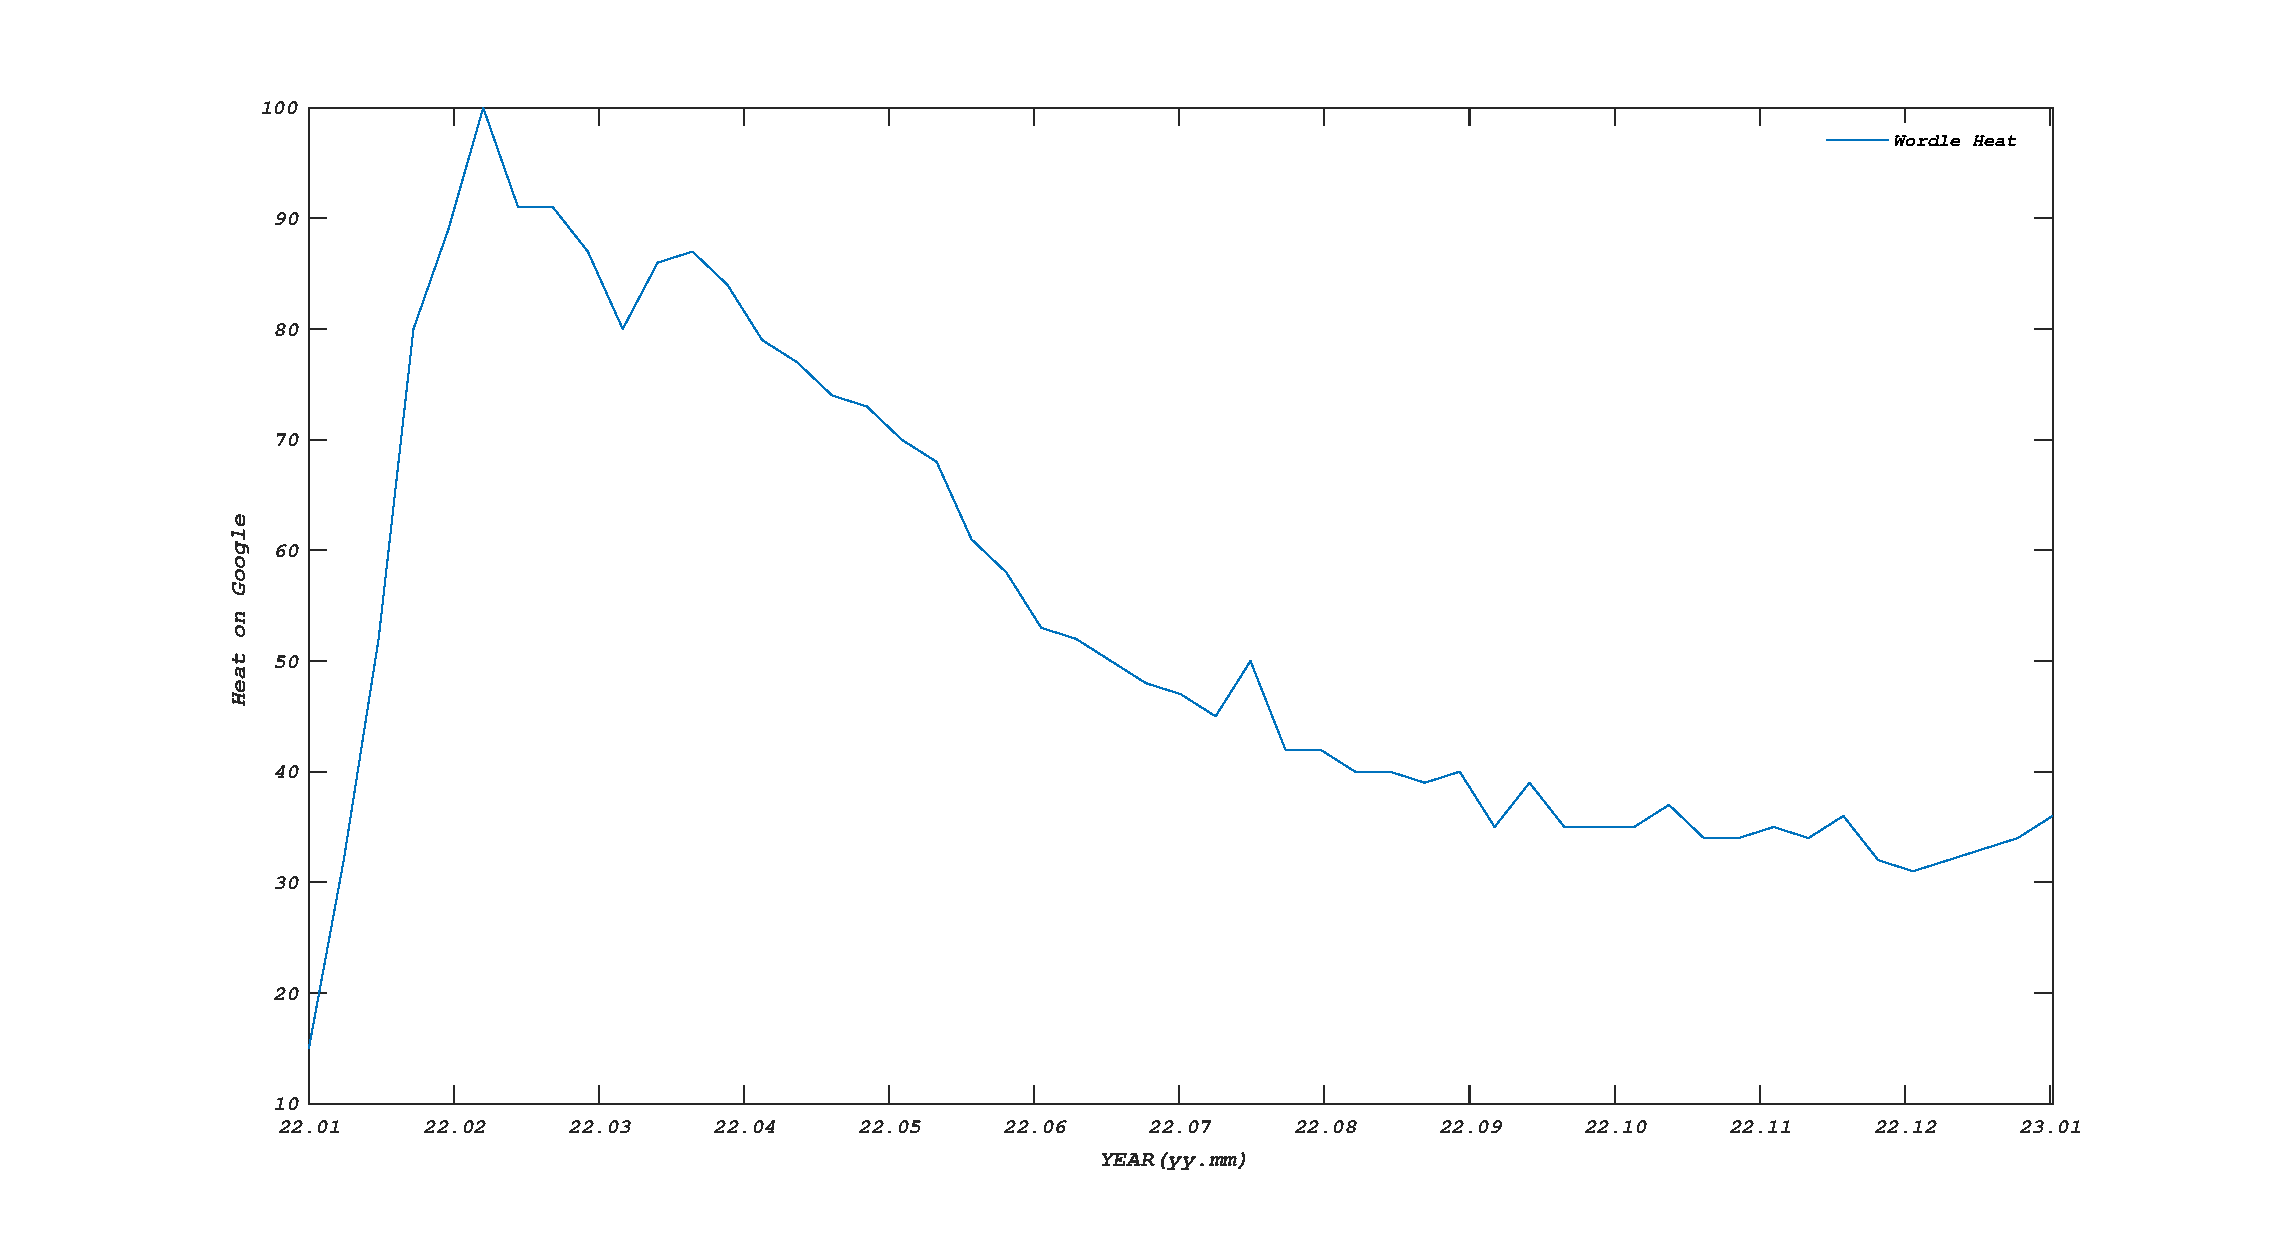
\includegraphics[width=\textwidth]{img/heat.eps}
% \caption{heat}
% \end{figure}
% \begin{figure}[htbp]
% \centering
% 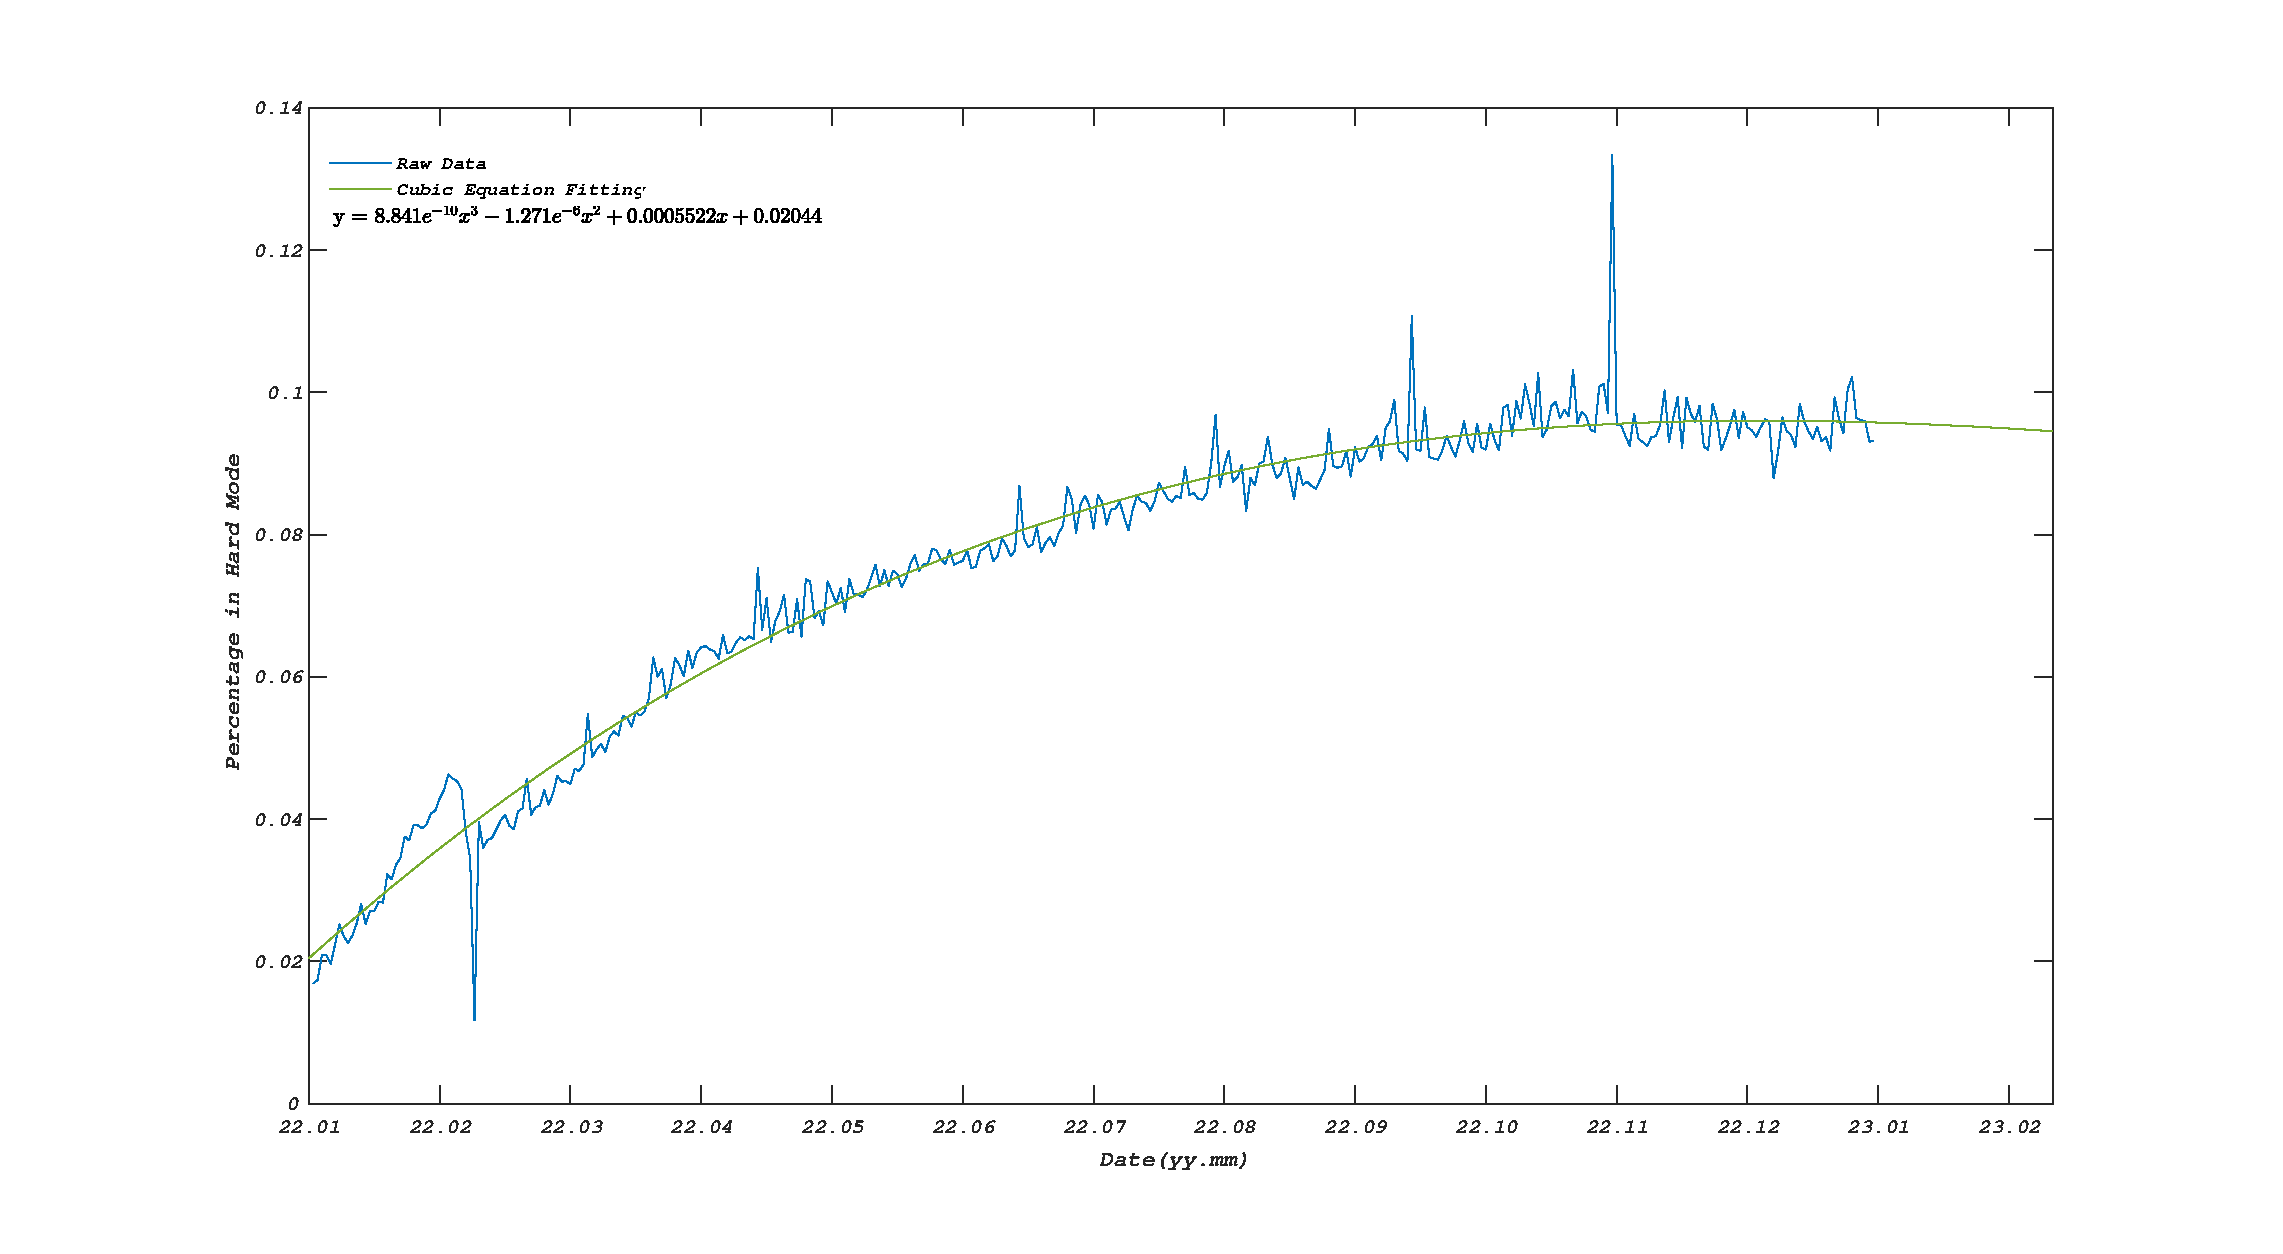
\includegraphics[width=\textwidth]{img/sanci.eps}
% \caption{sanci}
% \end{figure}
% \begin{figure}[htbp]
% \centering
% 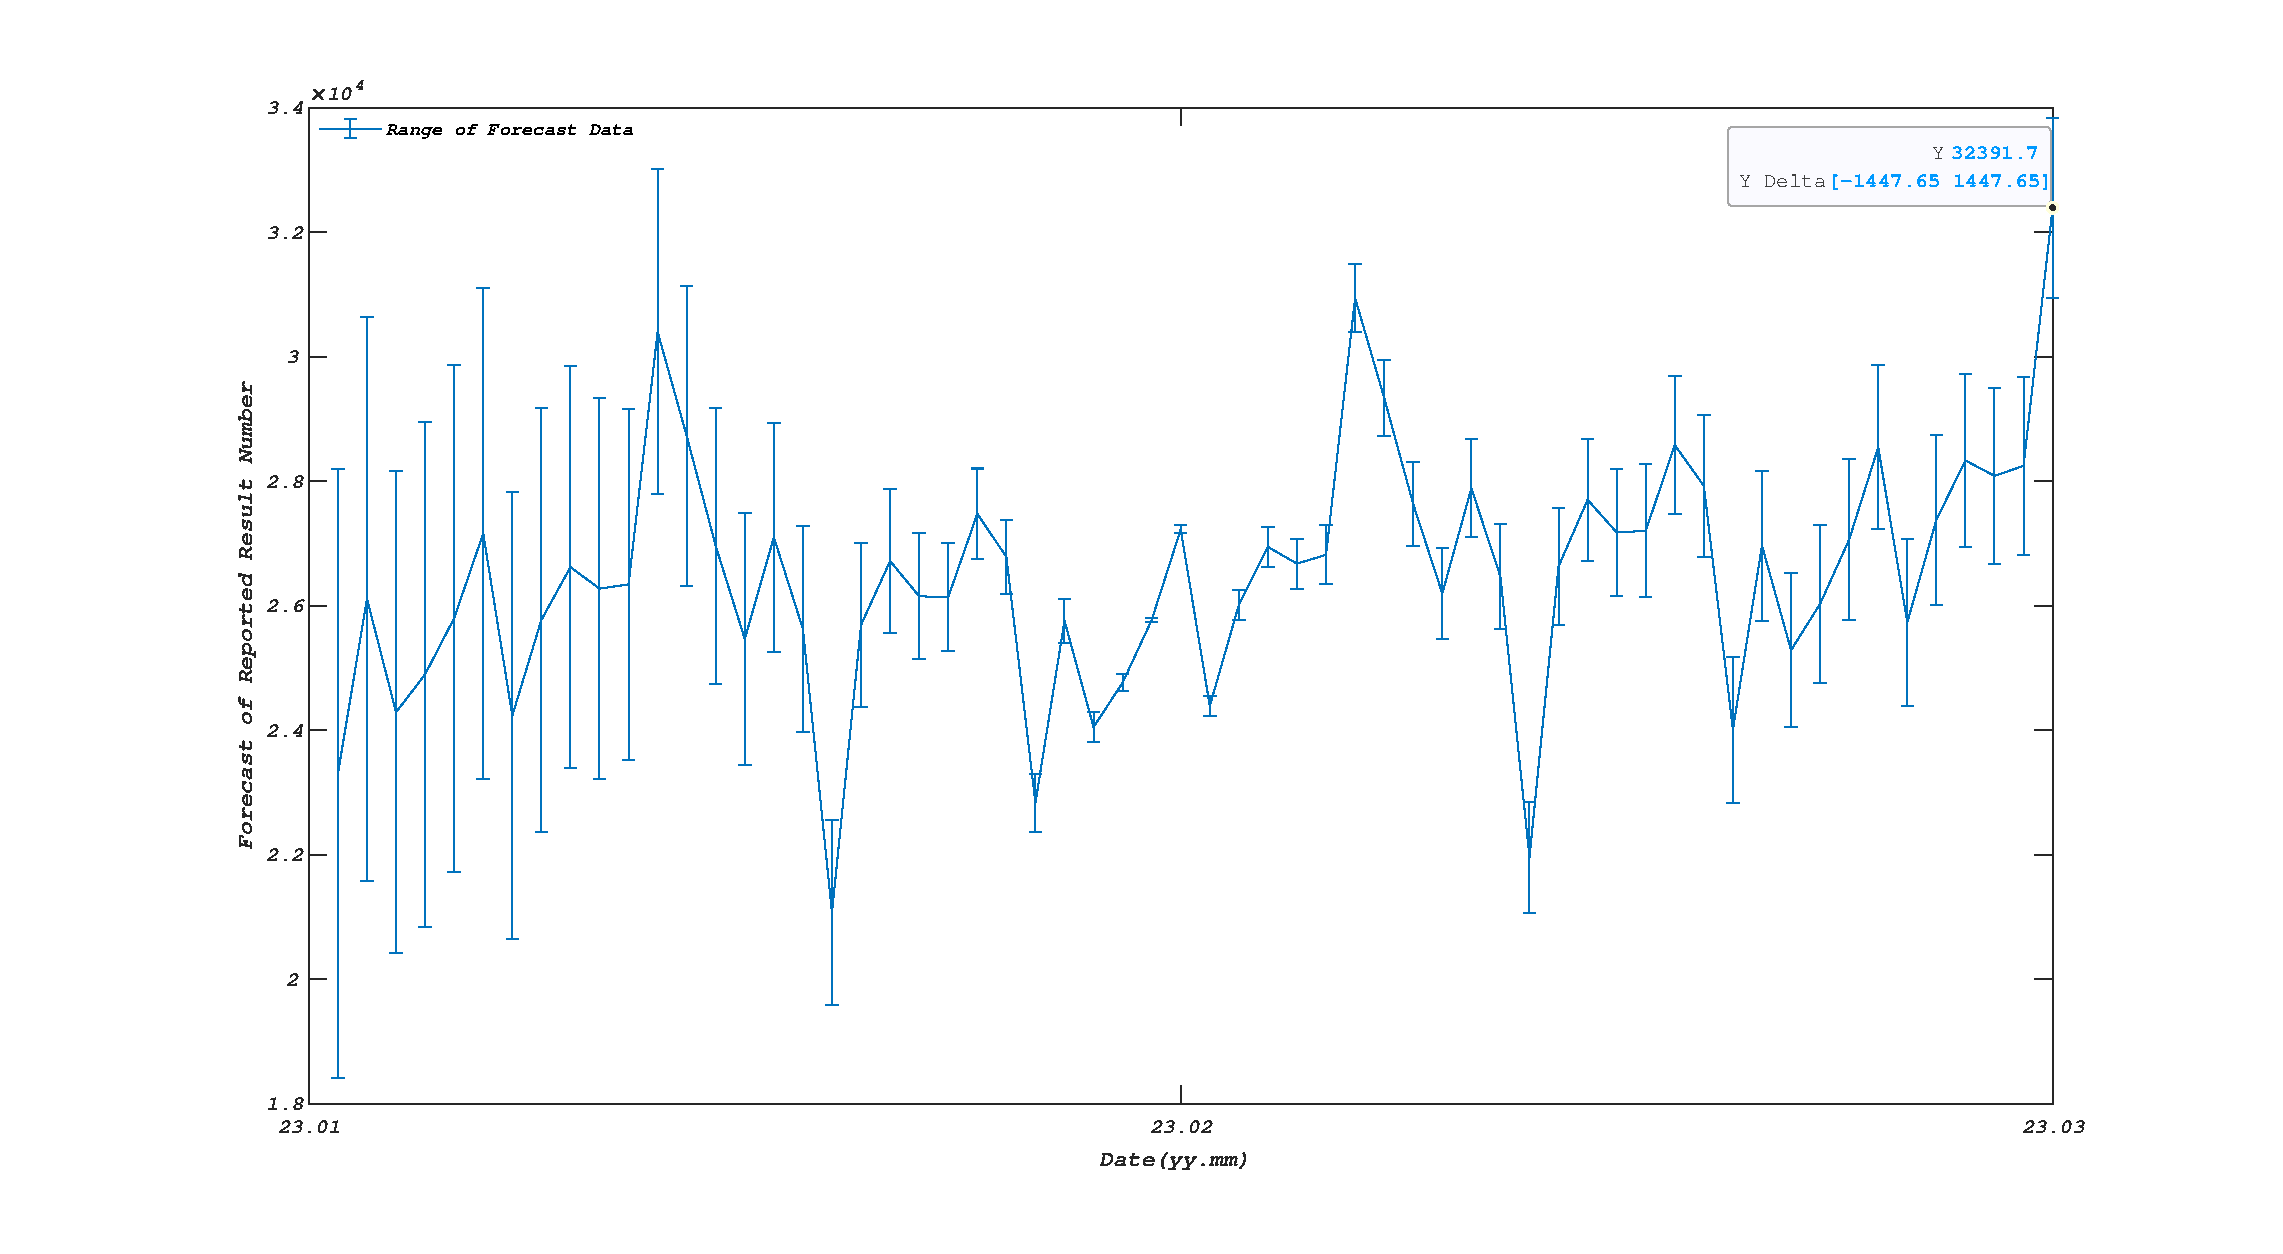
\includegraphics[width=\textwidth]{img/wucha.eps}
% \caption{wucha}
% \end{figure}
% \begin{figure}[htbp]
% \centering
% 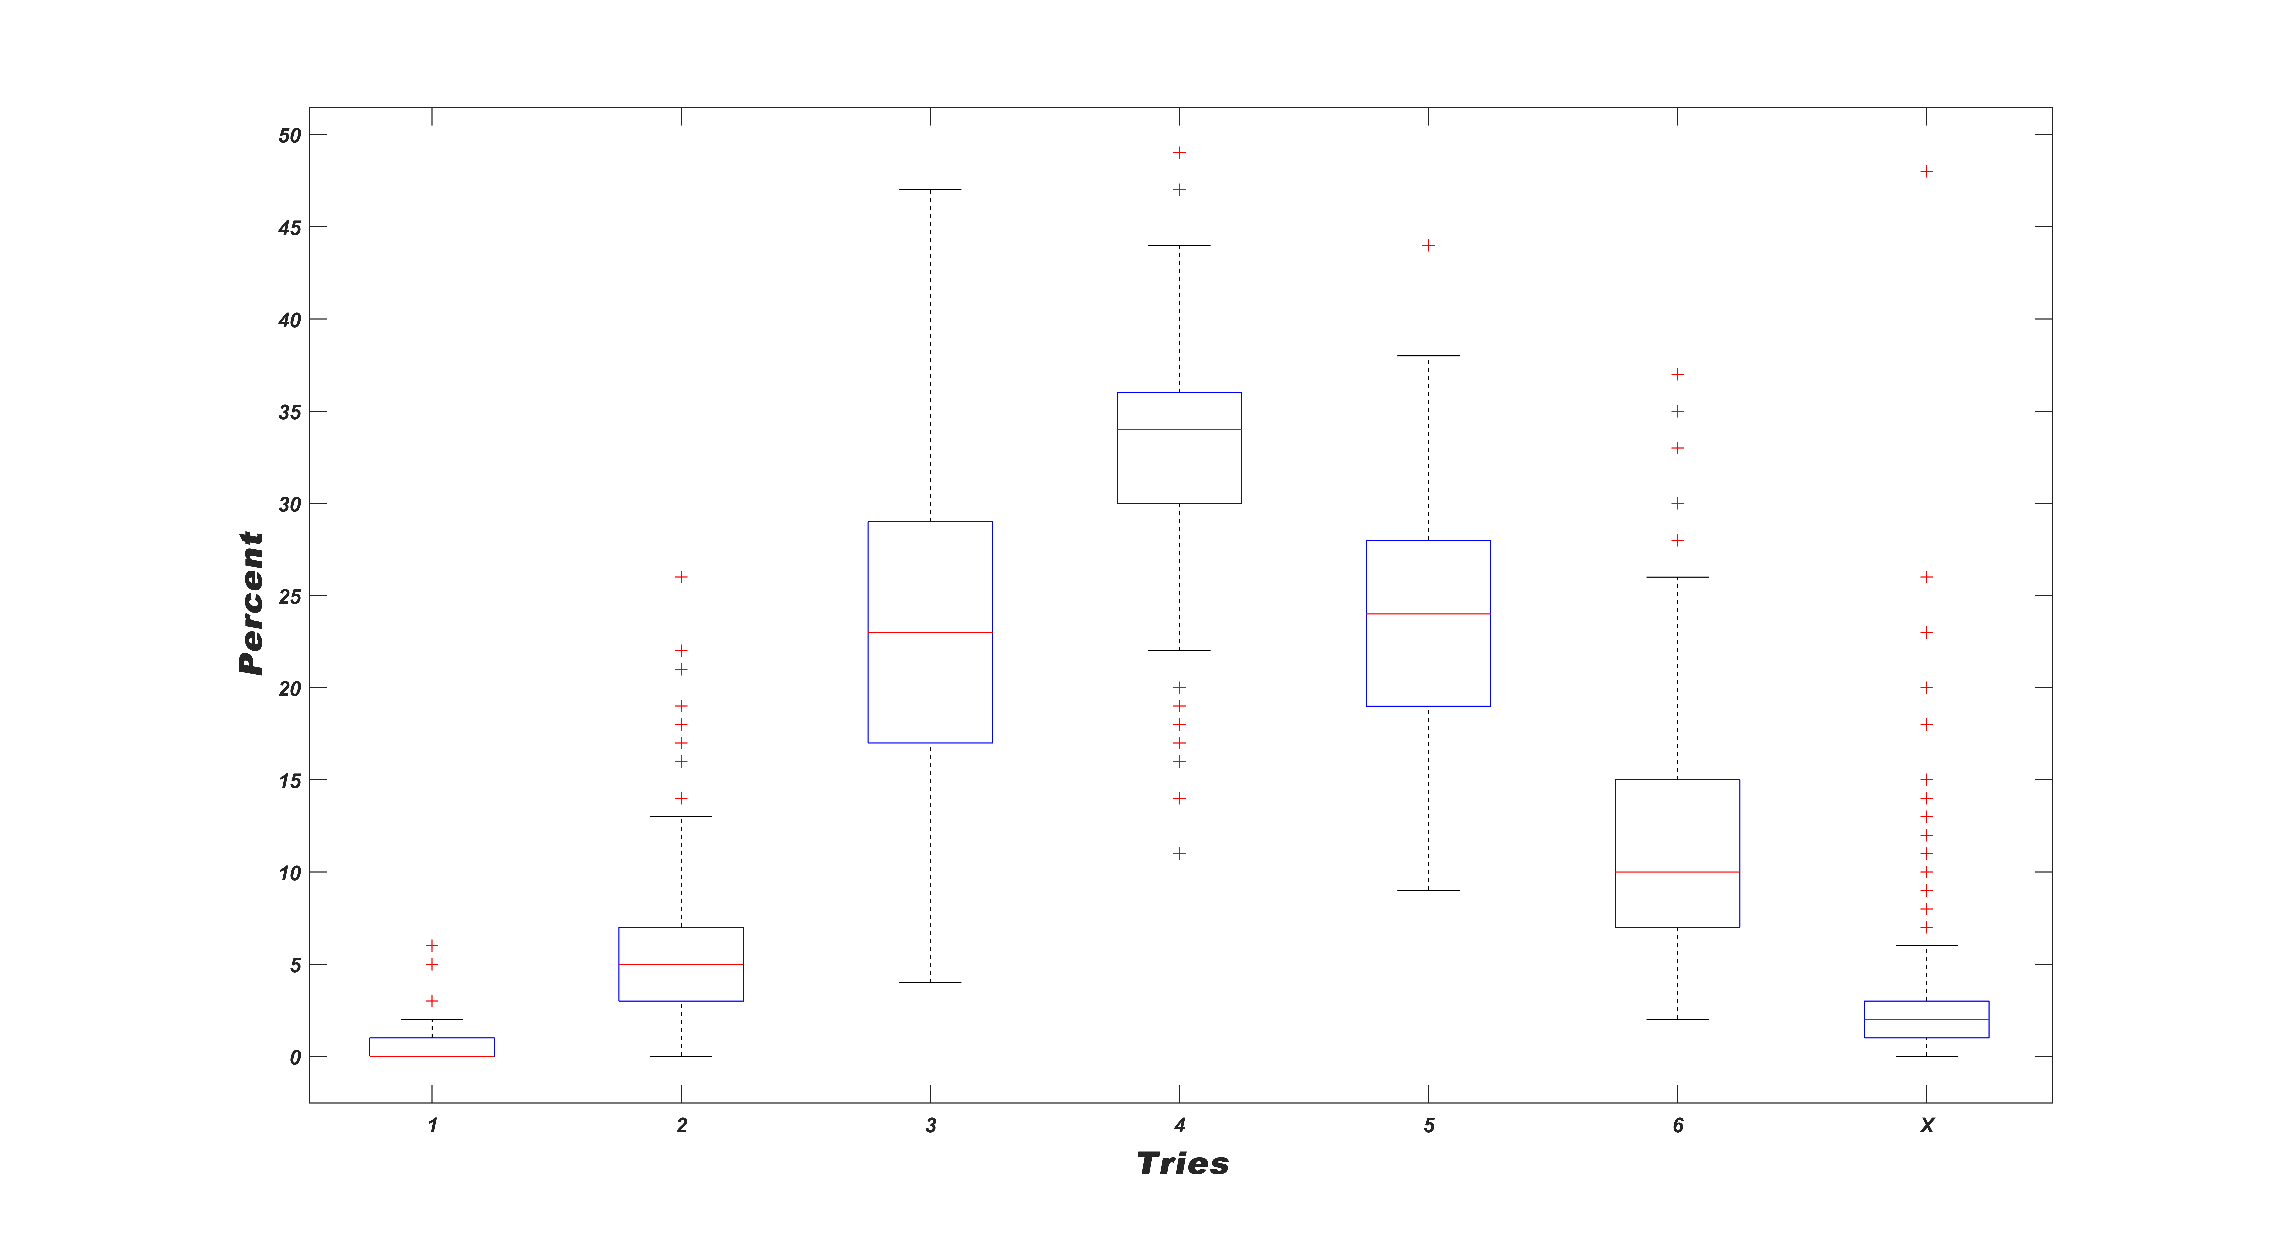
\includegraphics[width=\textwidth]{img/xxt.eps}
% \caption{xxt}
% \end{figure}
% \begin{figure}[htbp]
% \centering
% \begin{subfigure}[b]{.49\textwidth}
% 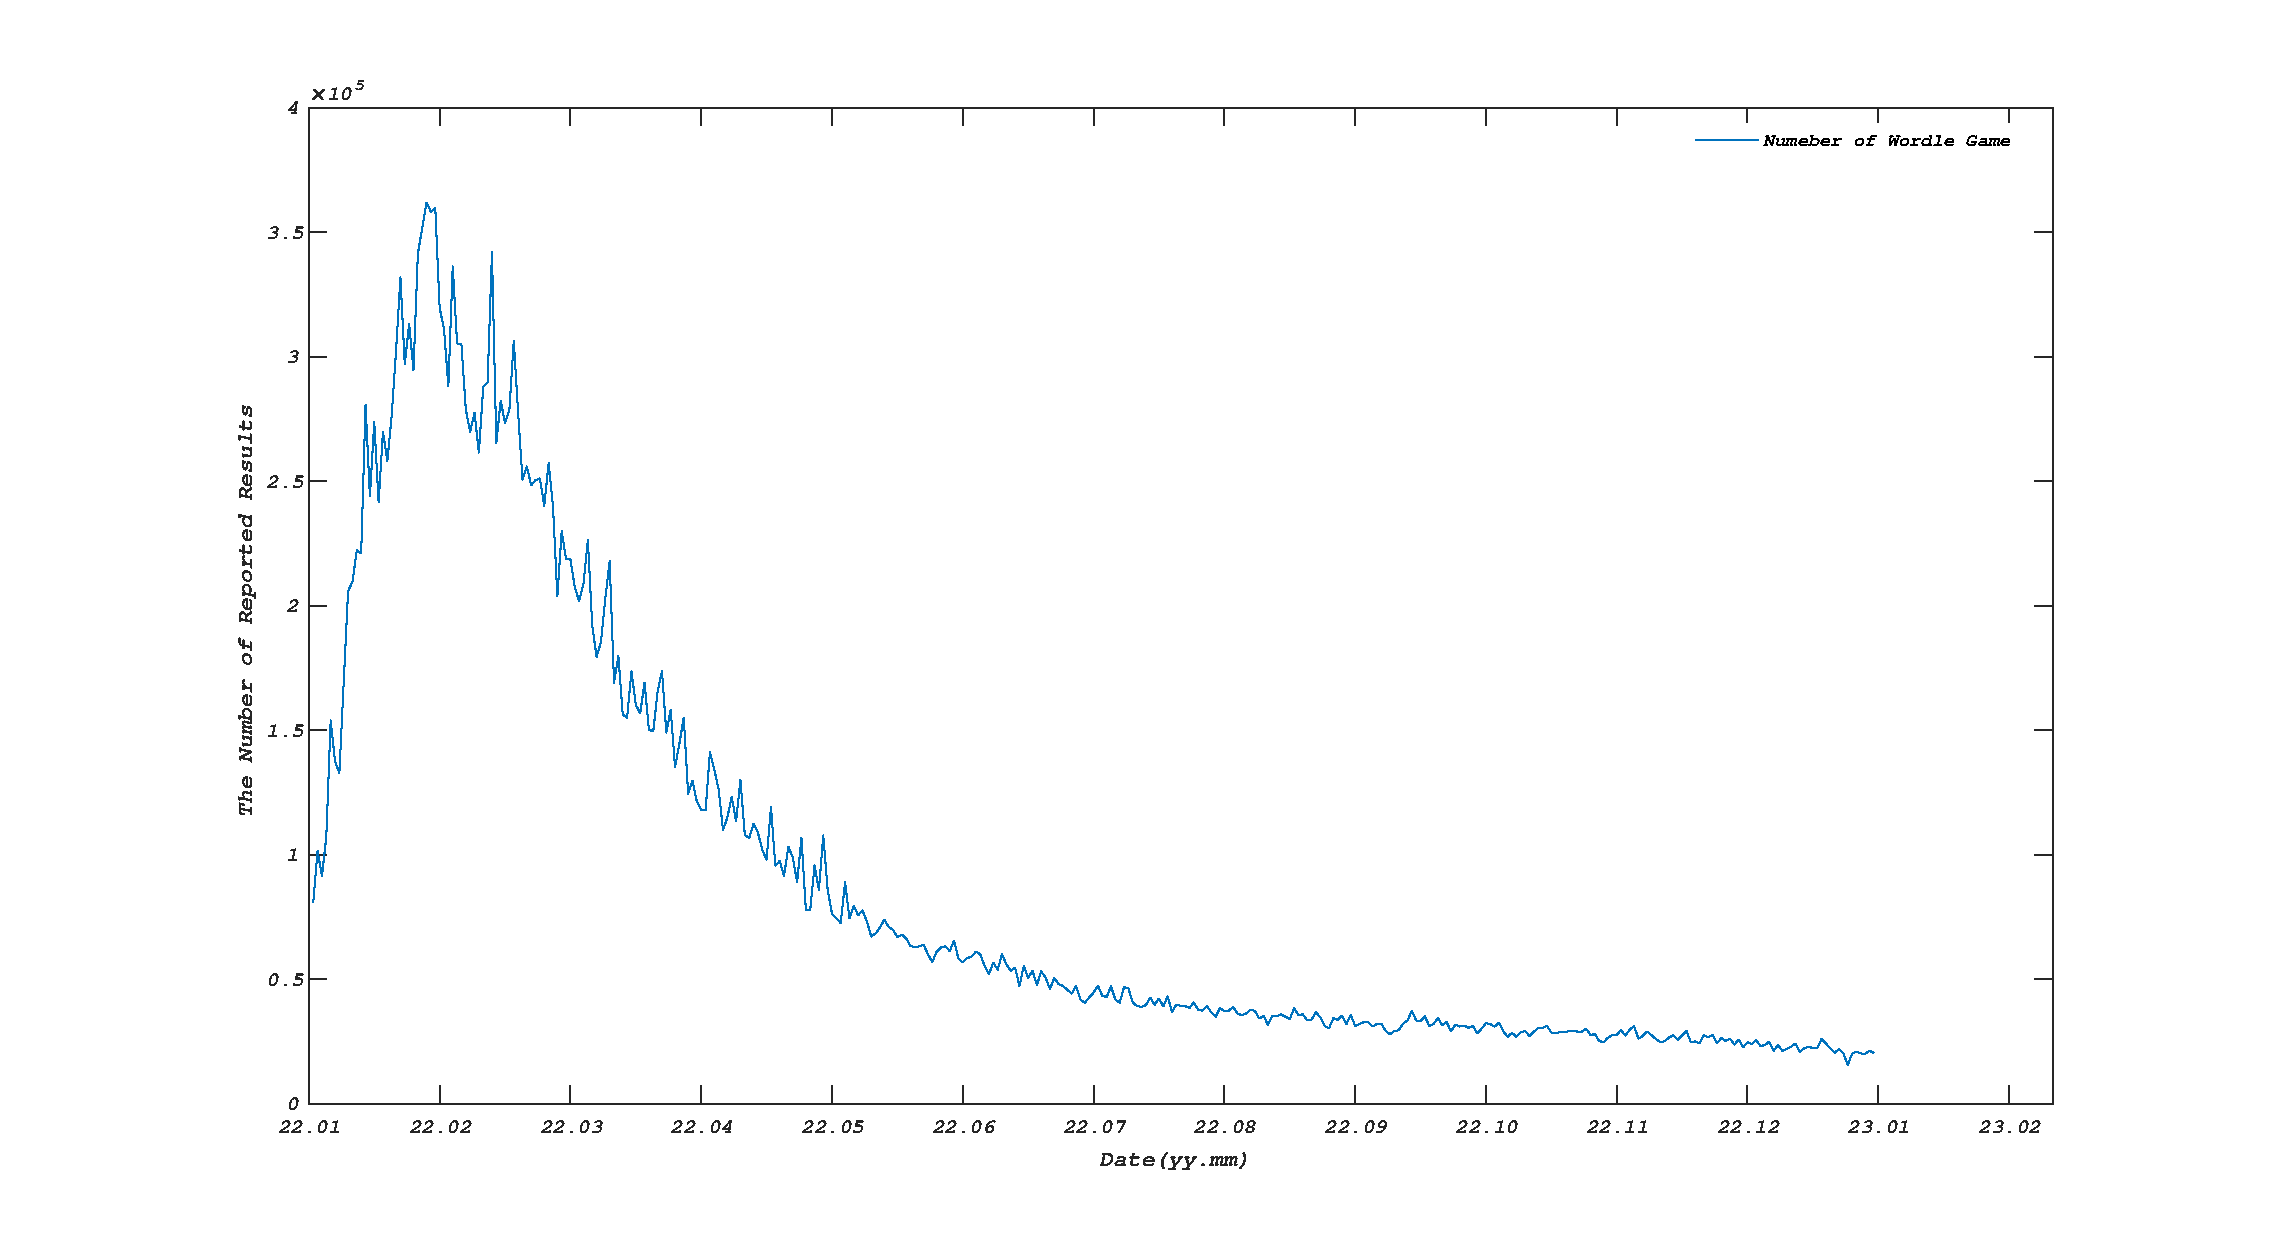
\includegraphics[width=\textwidth]{img/yuanshi.eps}\caption{The Number of Reported Results}
% \end{subfigure}
% \begin{subfigure}[b]{.49\textwidth}
% 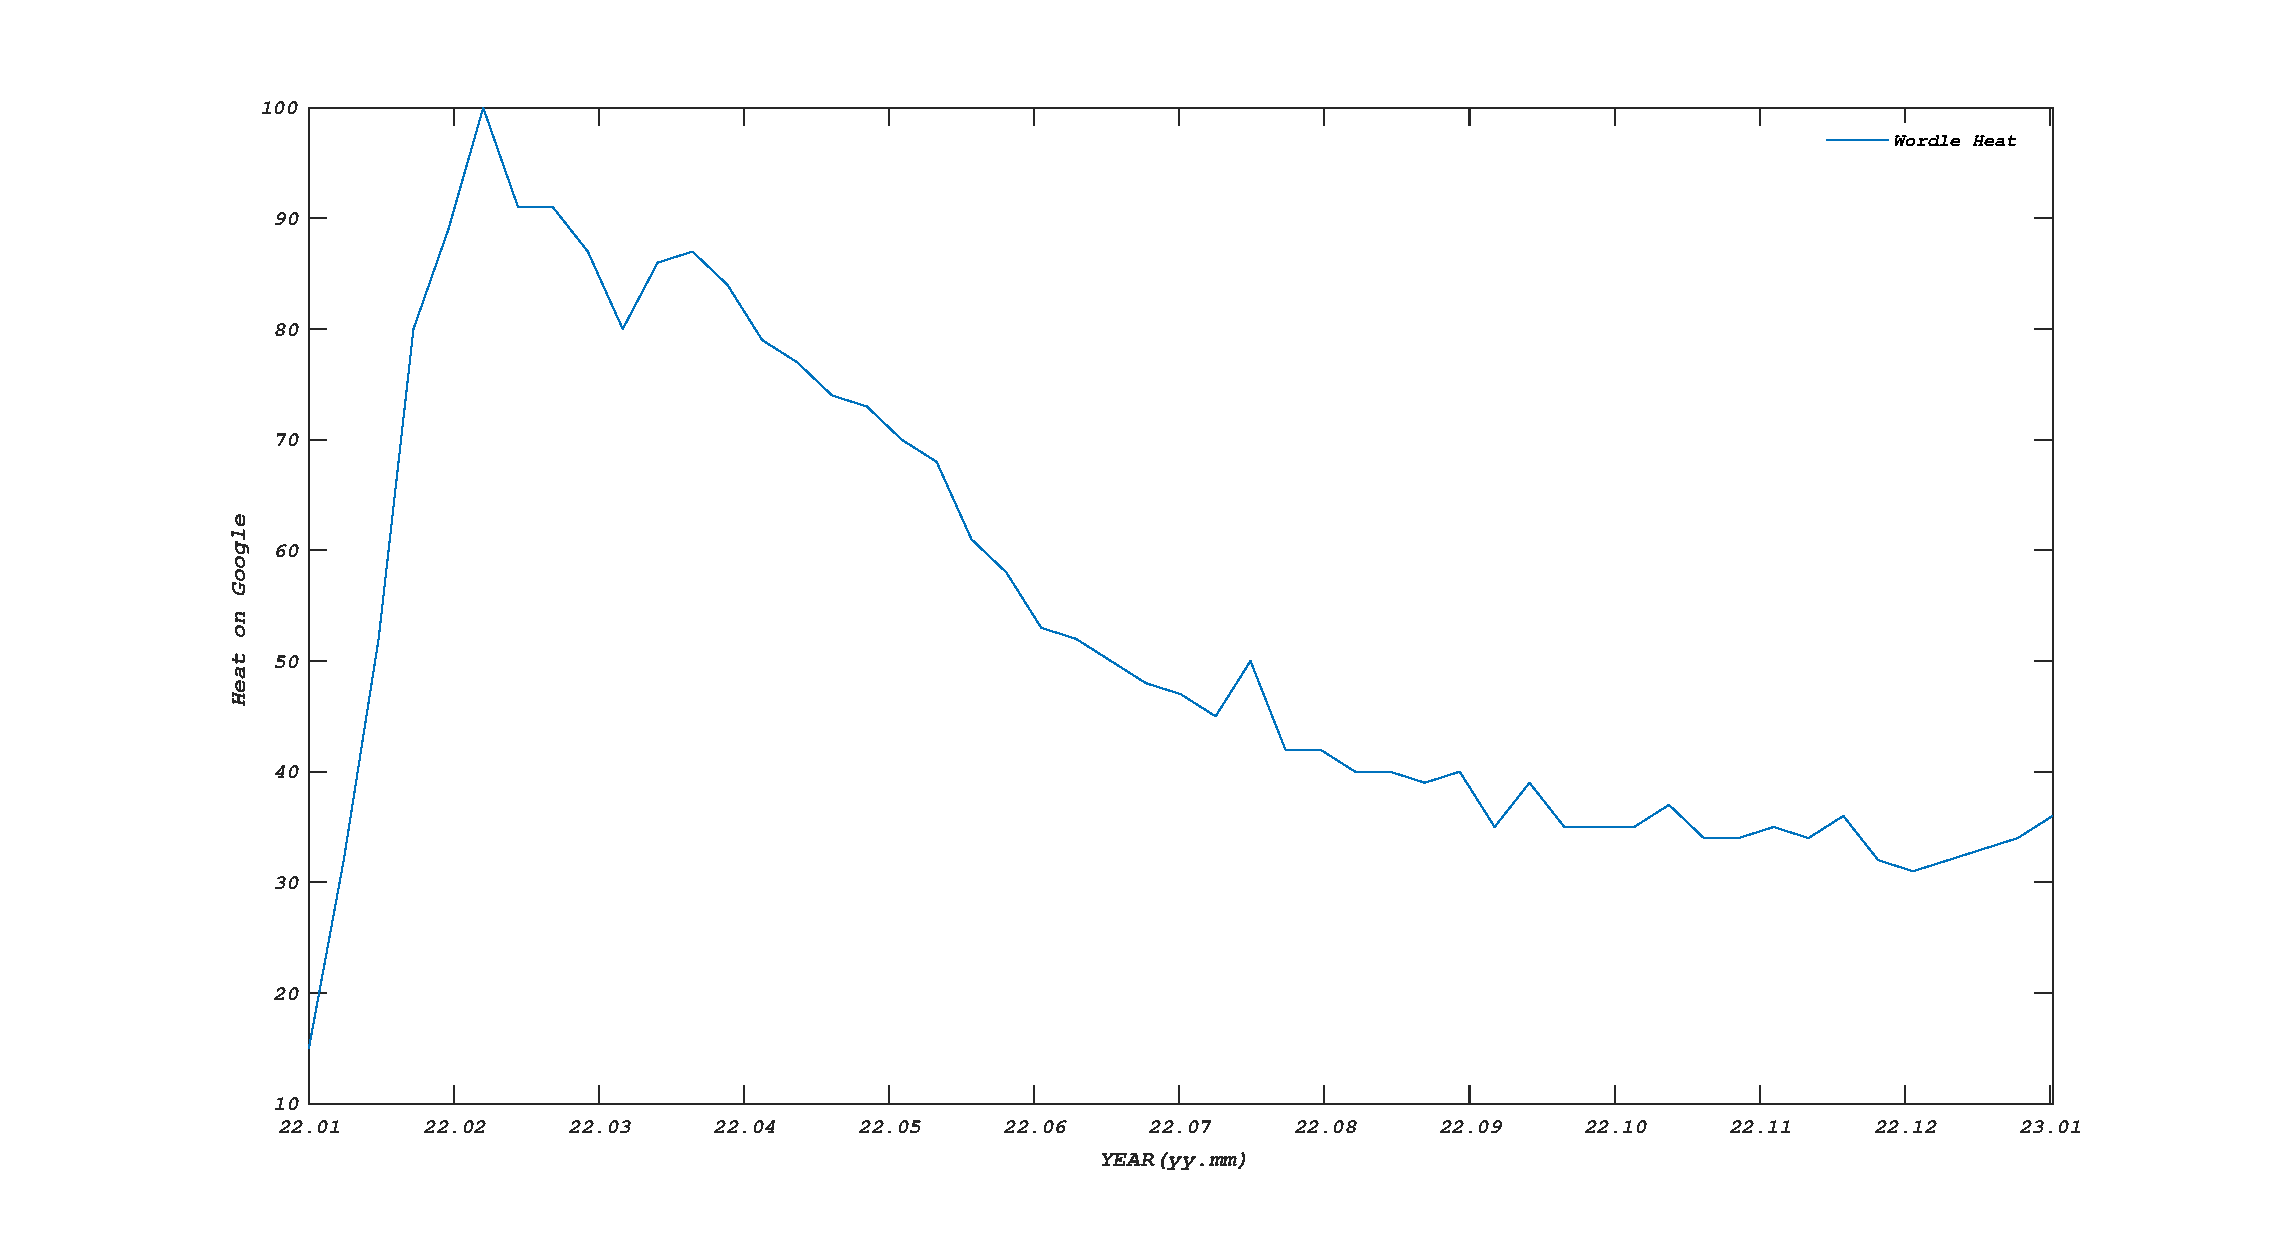
\includegraphics[width=\textwidth]{img/heat.eps}\caption{Heat on Google}
% \end{subfigure}
% \caption{Changing Trend of Number and Heat}\label{Changing Trend of Number and Heat}
% \end{figure}
\section{Assumptions and Notations}
\subsection{Assumptions}
To simplify our model, this paper makes following basic assumption, each of which is properly
justified.
\begin{itemize}
	\item We assume that in the temporal prediction model of Task 1, the data set is only related to time, the effect of the words themselves on the prediction results is not considered.
\item We assume that the difficulty of the word is most correlated with the metric we selected, we do not consider the effect of factors other than word attributes on the percentage of each number of guessed words in the game.
\end{itemize}
\subsection{Notations}
Notations that we use in the model are shown in the Table \ref{tb:notation}:
% 三线表示例
\begin{table}[!htbp]
\begin{center}
\caption{Notations}
\begin{tabular}{clc}
	\toprule[1.5pt]
	% \multicolumn{1}{m{3cm}}
	{\centering {\itshape\textbf{Symbol}}}
	&
	% \multicolumn{1}{m{8cm}}
	{\itshape\textbf{Description}}&{\centering {\itshape\textbf{Unit}}} \\
	\midrule
	AIC&Akaike Information Criterion&- \\
	SC&Schwarz Criterion&-\\
	MAPE&Mean Absolute Percentage Error&-\\
	RMSE&Root Mean Square Error&-\\
	\bottomrule[1.5pt]
\end{tabular}\label{tb:notation}
\end{center}
\end{table}











\section{{\sc \textbf{Task 1}}: The Number of Predicted Reported Results}
In order to analyze and predict the number of reported results, we cleaned the data (it includes for words with incorrect number of three letters and removal of outliers from the data), and we considered the number of reports related to the Hot of the game. We represented the number of searches for ``WORDLE'' in Google as the game's hotness. They are listed in the following Figure:
\begin{figure}[htbp]
\centering
\begin{subfigure}[b]{.49\textwidth}
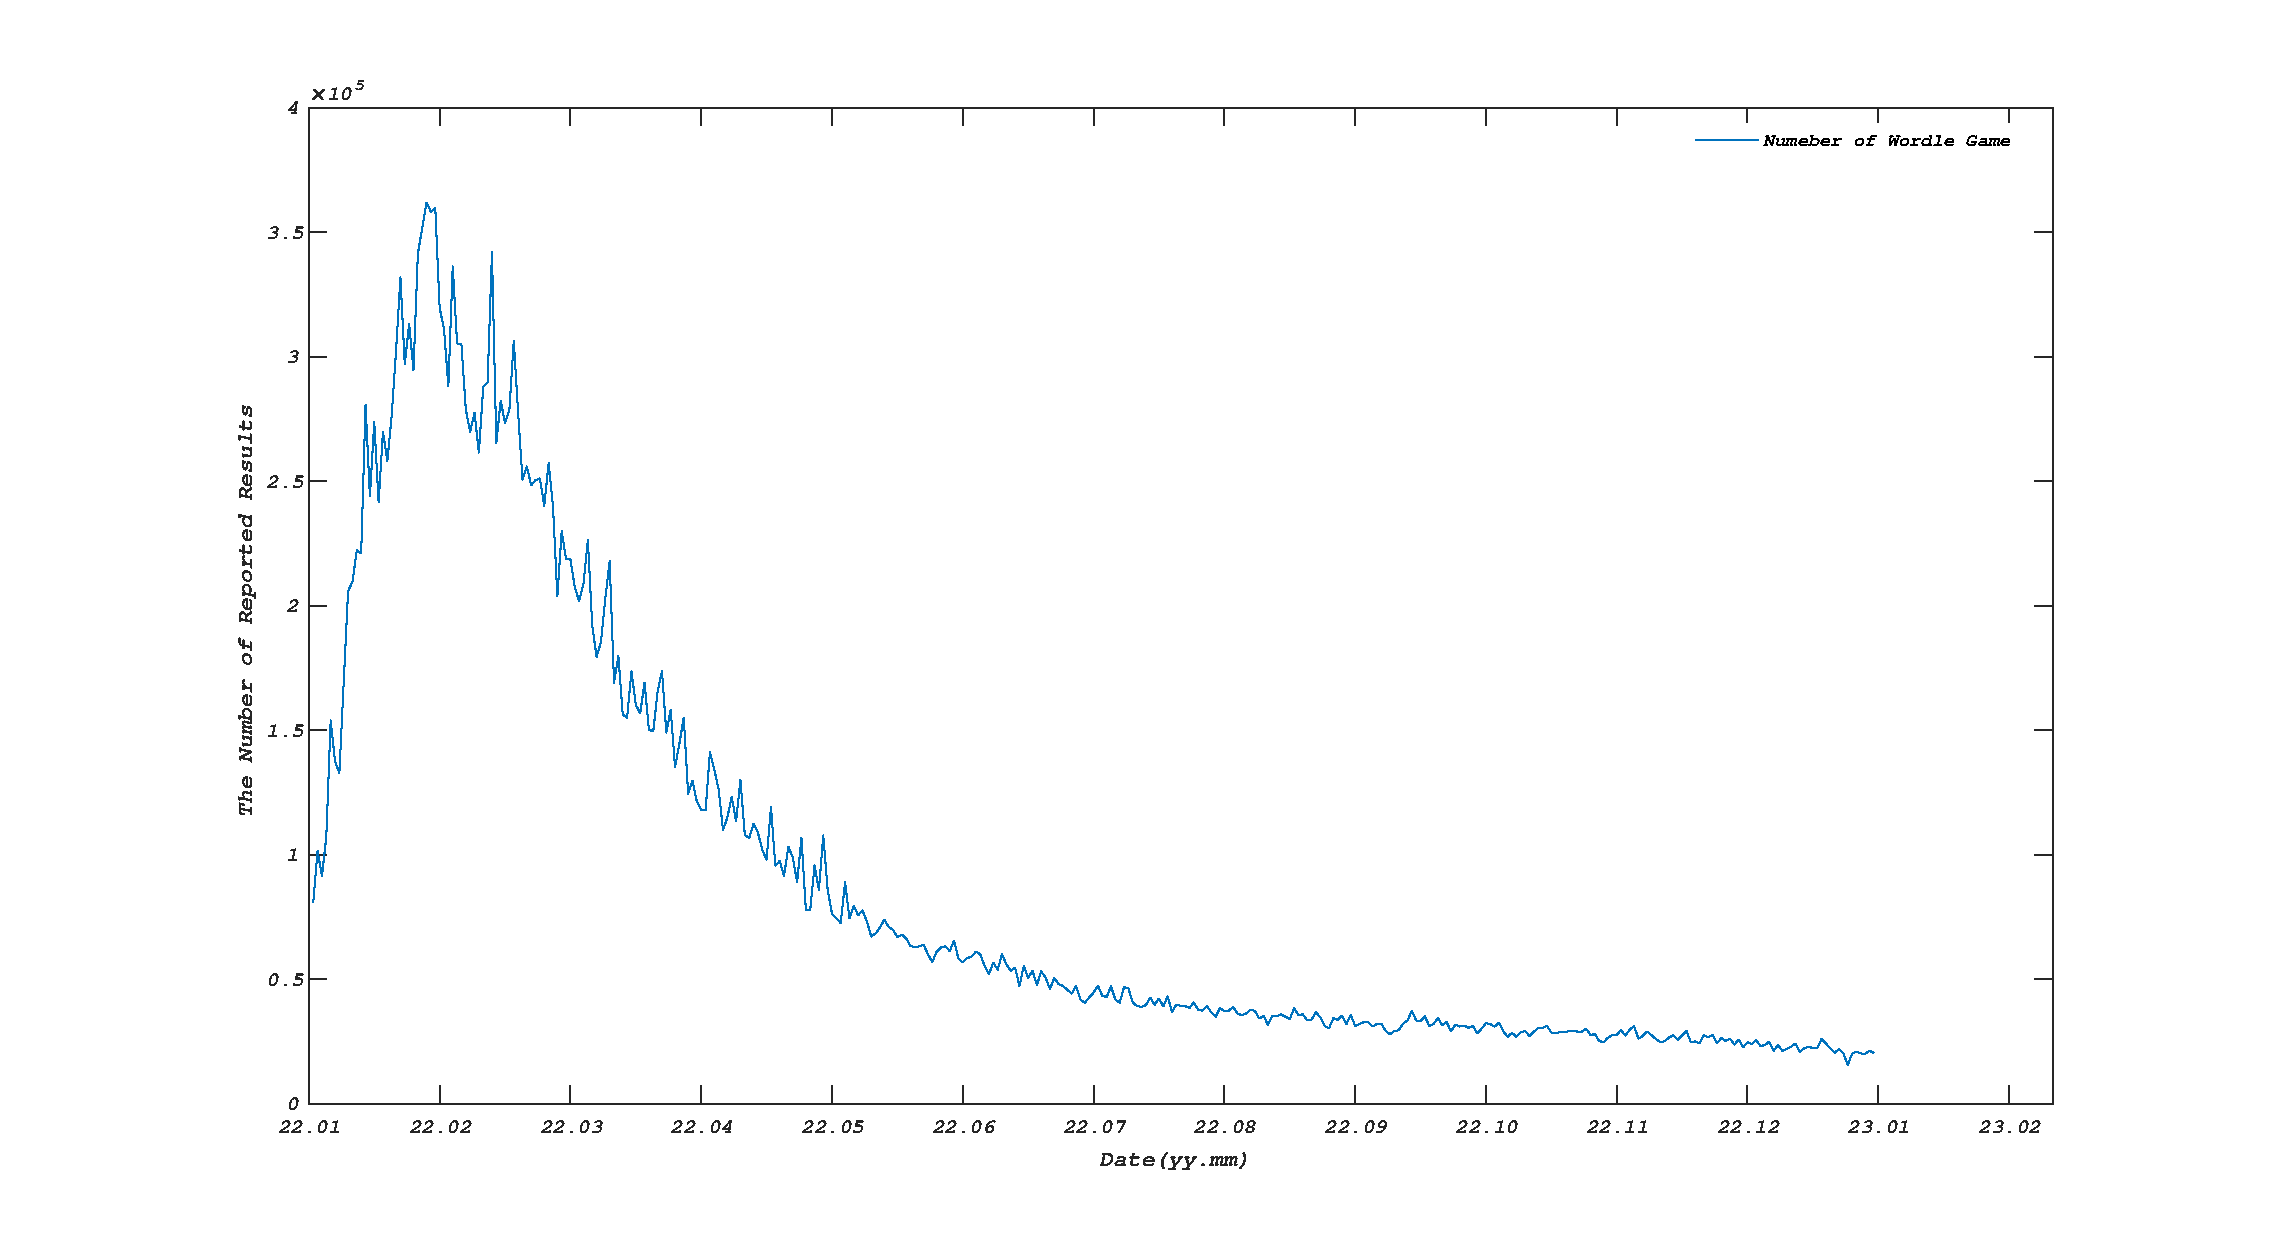
\includegraphics[width=\textwidth]{img/yuanshi.eps}\caption{The Number of Reported Results}
\end{subfigure}
\begin{subfigure}[b]{.49\textwidth}
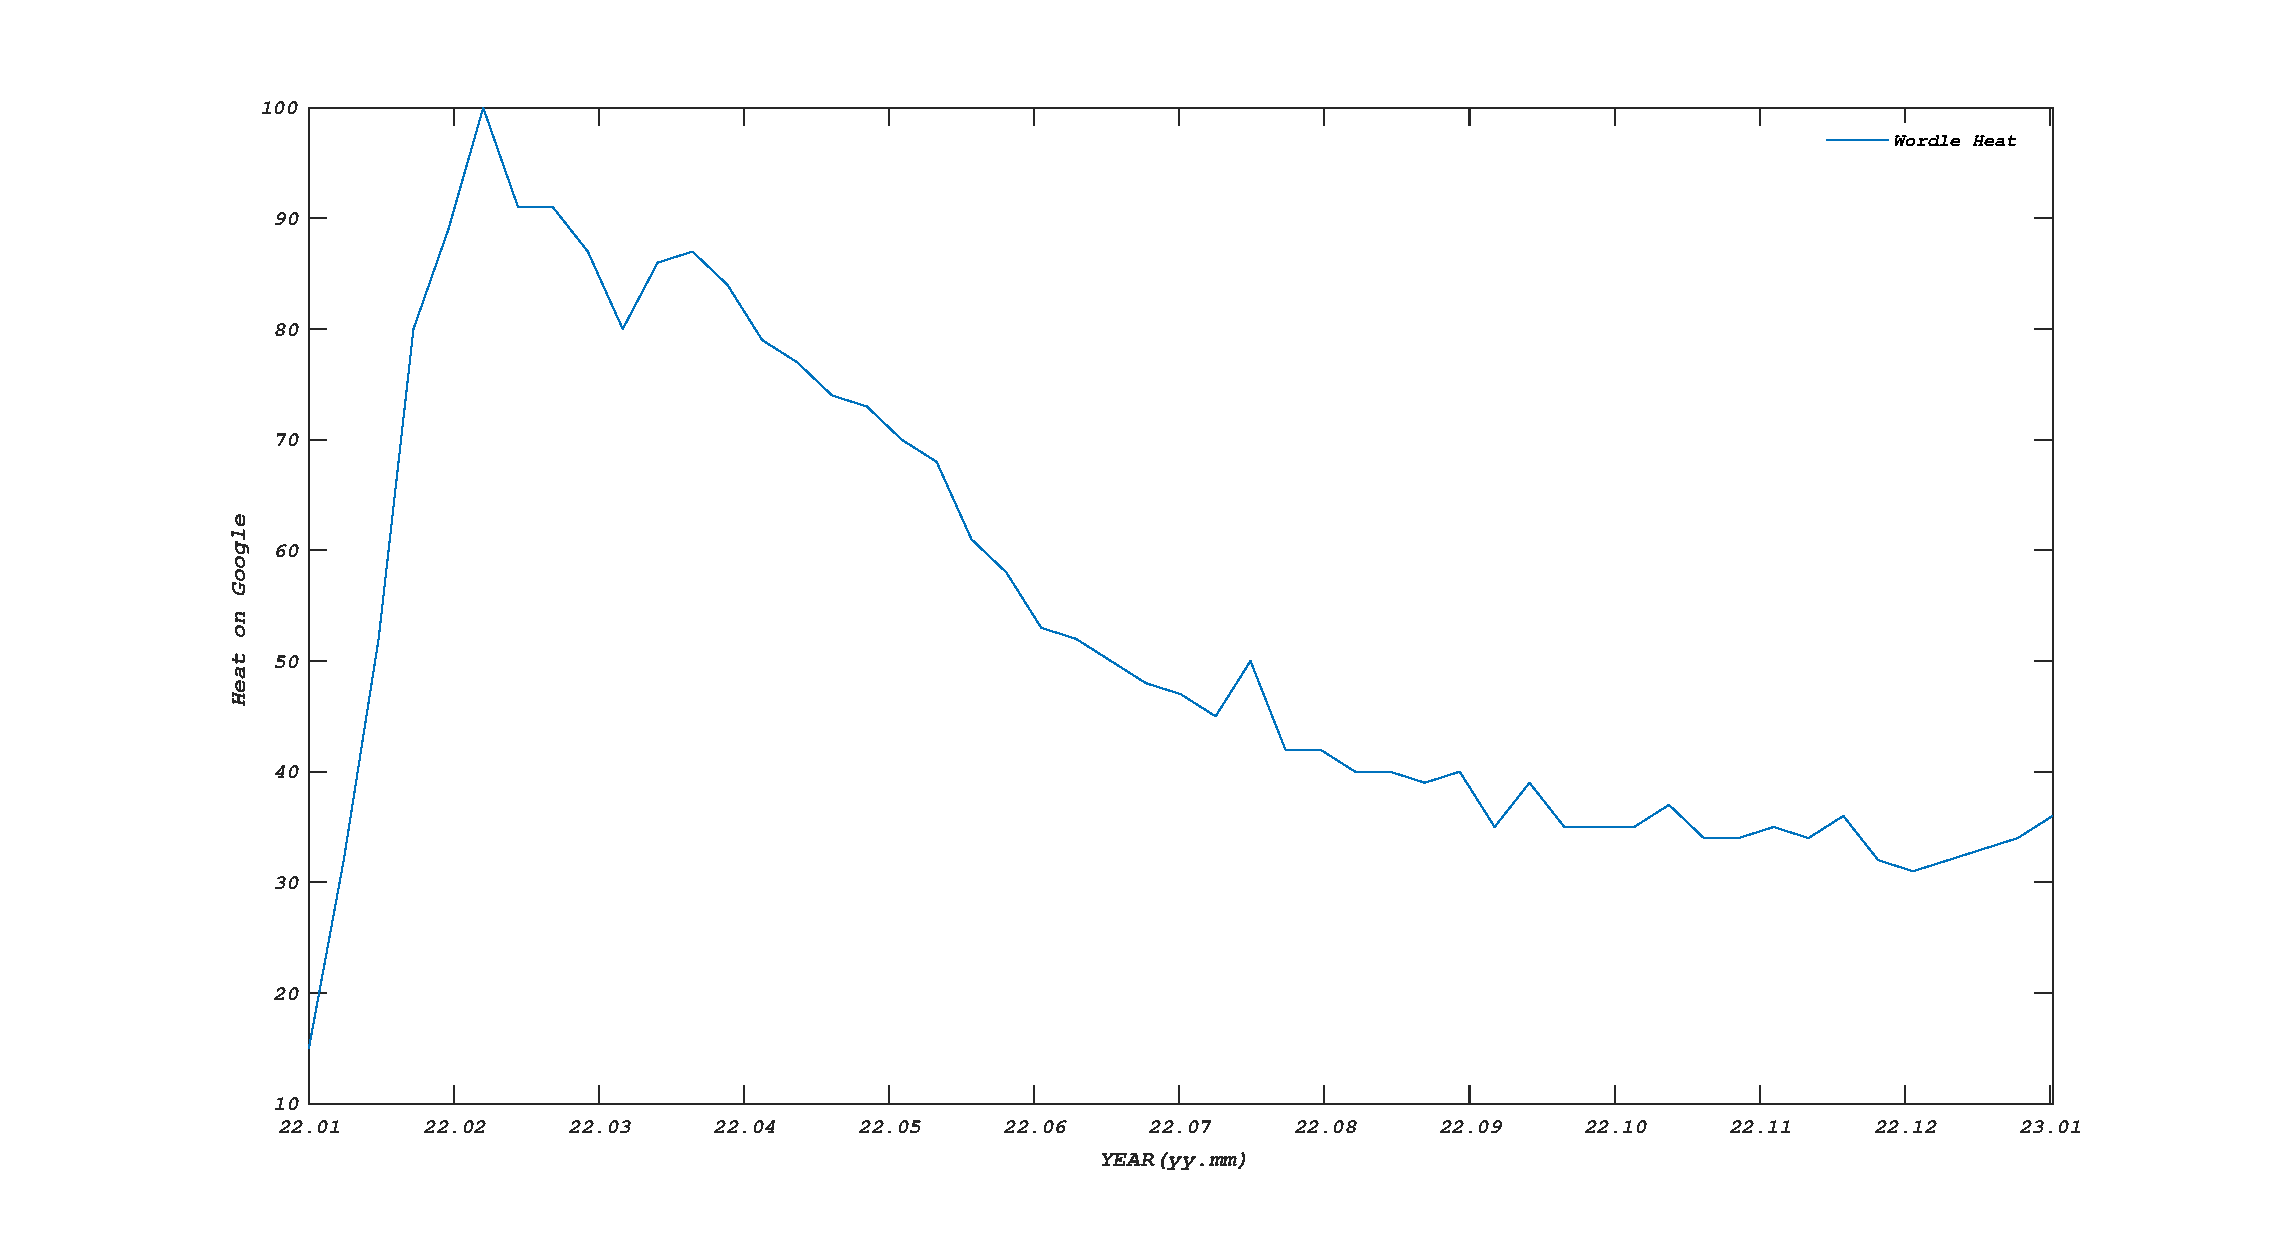
\includegraphics[width=\textwidth]{img/heat.eps}\caption{Hotness on Google of ``WORDLE''}
\end{subfigure}
\caption{Changing Trend of Number and Heat}\label{Changing Trend of Number and Heat}
\end{figure}

So we can easily get a preliminary conclusion: the number of reported results changes with the change in the heat of ``WORDLE'' on Google, and there is a positive correlation between the two before. We this explains the reason for the change in the number of reported results: because of the change in the heat of the game. Of course this is only a simple model, in order to get a concrete picture of how the number of reports changes and how the number of reports will change in the future, we will build a mathematical model below and get the number of reports in the interval of March 1, 2023.
\subsection{Percentage of Difficult Mode}
To find out whether the properties of the word itself affect the percentage of people playing in difficult mode, we first assume that there is no correlation between the two. We plot the percentage of people playing in difficult mode versus time, and to show this percentage more visually over time, we fit a cubic polynomial to it and shown that in Figure \ref{sancinihe}:
\begin{figure}[htbp]
\centering
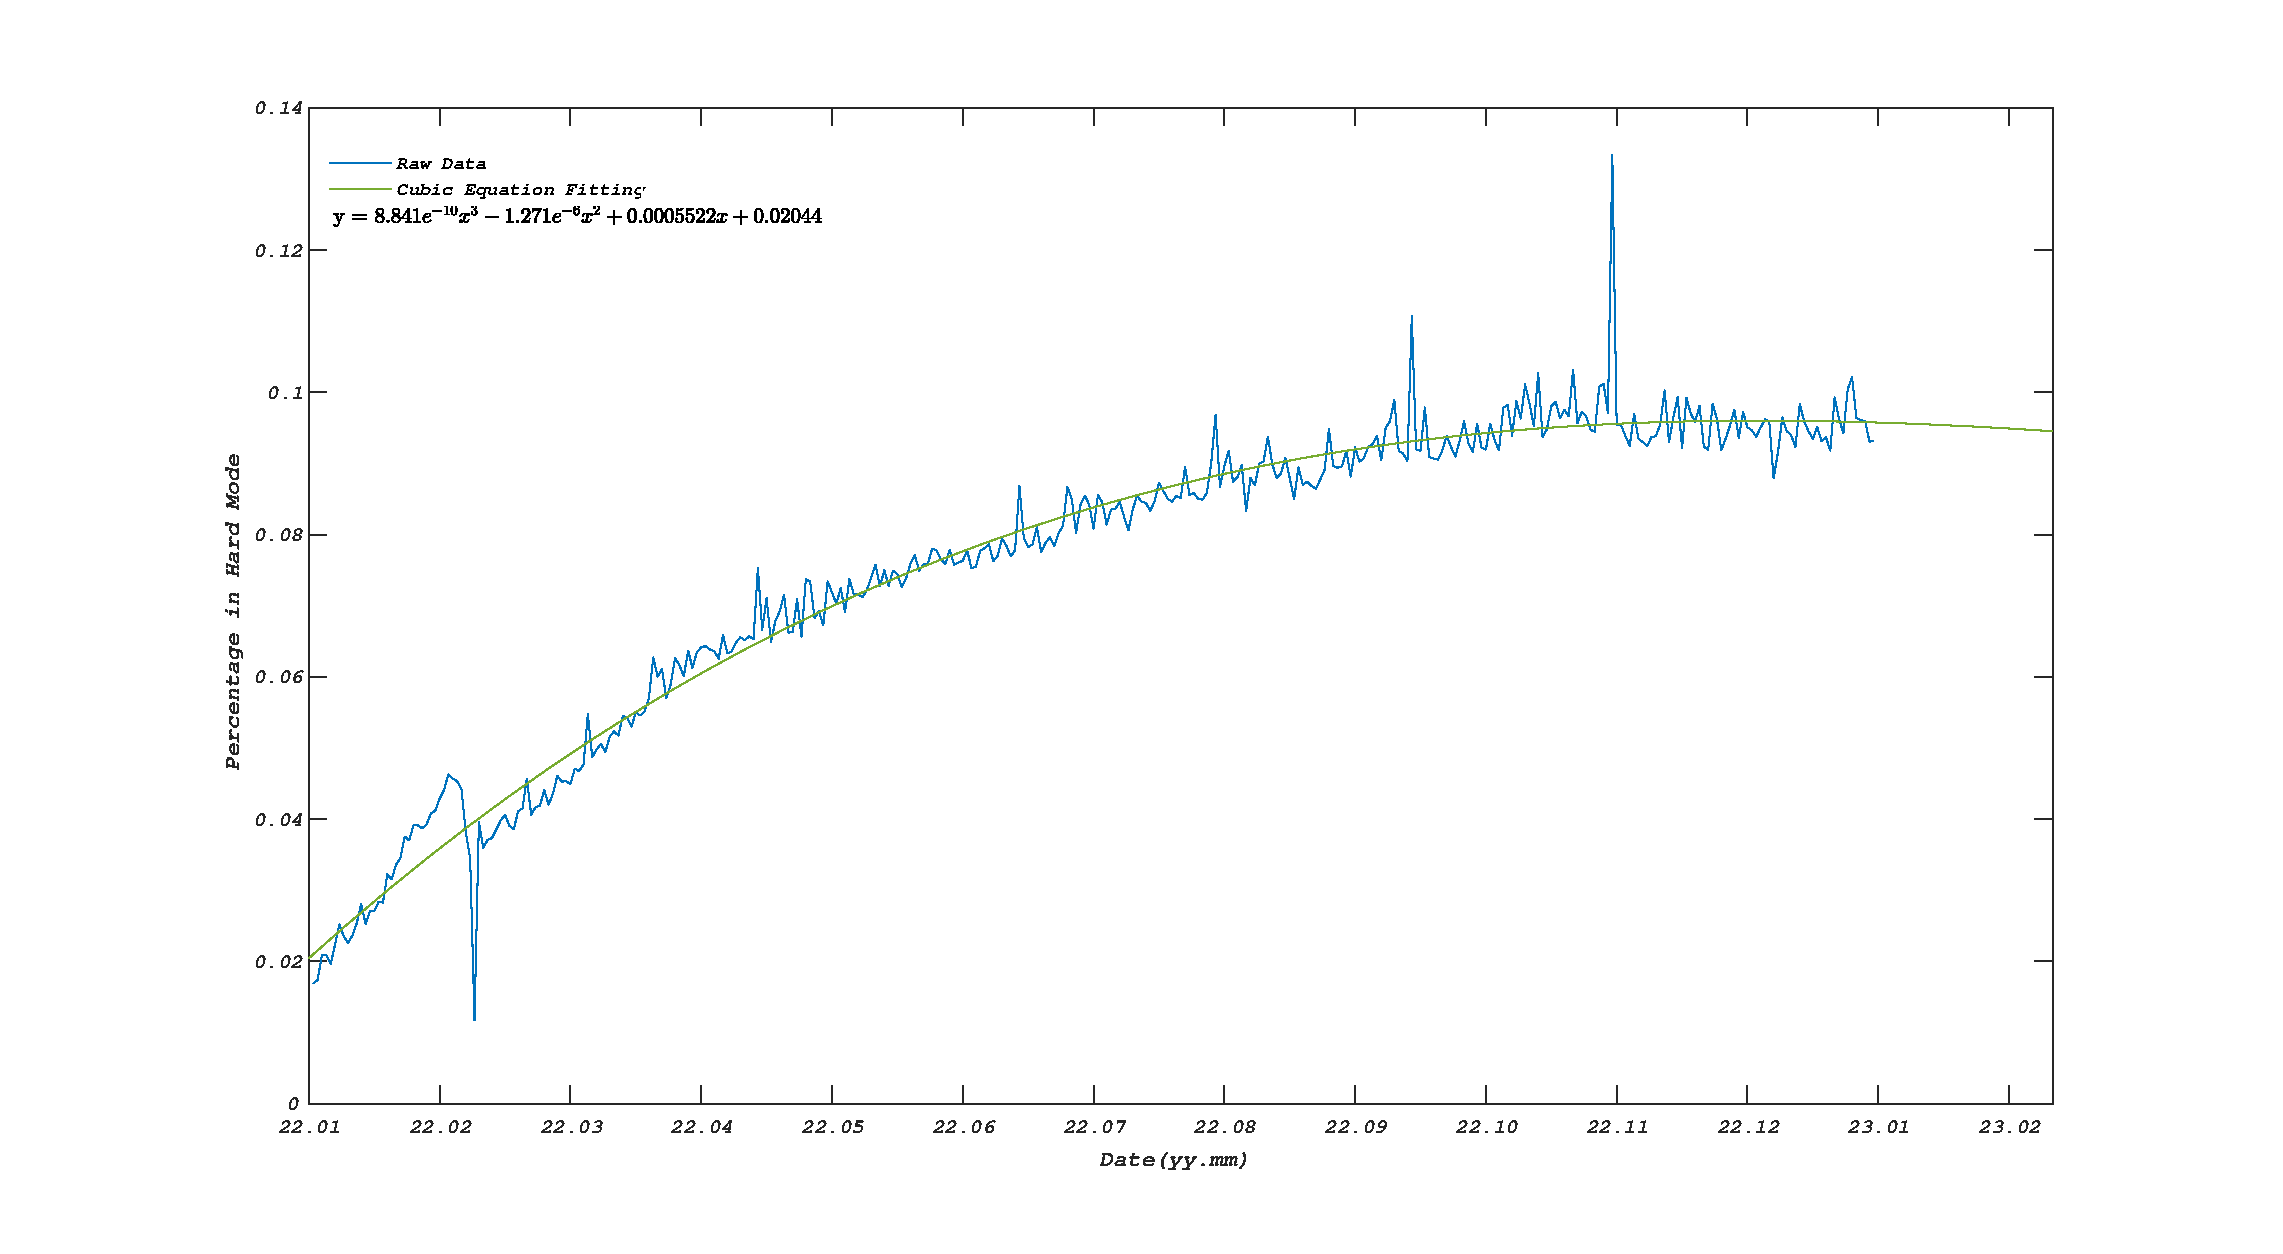
\includegraphics[width=\textwidth]{img/sanci.eps}
\caption{Cubic Polynomial Fitting}\label{sancinihe}
\end{figure}

We found that the percentage of people playing in the difficult mode basically obeyed the distribution of the cubic polynomial $y=8.841e^{-10}x^3-1.271e^{-6}x^2+0.0005522x+0.02044$($R^2$ reached 0.9681, and the Residual Norm was only 0.07525), and the words were given completely randomly, not with We therefore believe that the percentage of people playing the game in difficult mode is not related to the nature of the words themselves. The reason for this is that we are not told in advance that the word is more difficult and we are advised not to enable hard mode or we are told that the word is easier and we are forced to open hard mode in order to increase the playability of the game: this is certainly not possible. We would venture to guess that the increase in the number of people choosing to play in hard mode is due to the increased popularity of the game and the fact that they are actively choosing hard mode in order to be able to ``show off'' their ``battle results'' on Twitter (Of course, this is just our guess, the actual situation may be very complicated, in fact, people's thoughts cannot be completely unified).
\subsection{Establishment of ARIMA Model}
\subsubsection{ARIMA Model Introduction}
The Autoregressive Integrated Moving Average model (\textbf{ARIMA}) is a type of time series forecasting model that allows us to transform our non-stationary time series into a stationary time series after finite difference processing. ARIMA is the most common in the series family due to the adaptability of linear patterns amongst
all time series strategies. Moreover, ARIMA model has the benefits of using a simpler algorithm and being
a studied technology in comparison to the second generation of forecasting methods which is the artificial neural
networks.
\subsubsection{Mathematical Modeling of ARIMA}
The mathematical model of ARIMA ($p, d, q$) is shown to be precise in the literature by combining AR ($p$)
and MA ($q$), While Integrated (\textbf{I}) reflects the separation of raw observations to allow the time series to become
stationary, the difference between the real data values, and the previous values are replaced with the data values.
The finite distinction of the data points in ARIMA ($p, d, q$) are used to transform the non-stationary time series to
the steady one. The mathematical formulation of ARIMA ($p, d, q$) is demonstrated as following Equations.
\begin{eqnarray}
	\varphi (L)(1-L)^dy_t & = & \theta (L)\varepsilon _t
\end{eqnarray}
\begin{eqnarray}
	(1-\sum_{i=0}^{p}\varphi _iL^i)(1-L)^dy_t=(1+\sum_{j=1}^q\theta_jL^j)\varepsilon_t
\end{eqnarray}
\begin{eqnarray}
	Y_t=\phi _0+\phi_1y_{t-1}+\phi_2y_{t-2}+\cdots +\phi_py_{t-p}+\varepsilon _t-\theta_1\varepsilon_{t-1}-\theta_2\varepsilon_{t-2}-\cdots-\theta_p\varepsilon_{t-p}
\end{eqnarray}
Where $y_t$ and $\varepsilon_t$ are the actual value and random error at time period $t$,respectively.$\varphi_1(i=1,2,\cdots ,p)$ and $\theta_j(j=0,1,\cdots ,q)$ are model paramenters. $p,d$ and $q$ are positive integers, referring to the order of the autoregressive, integrated, and moving average parts of the model, respectively. A typical method for identifying $p$ and $q$ is achieved by implementation of the Autocorrelation Function (\textbf{ACF}) and Partial Autocorrelation Functions (\textbf{PACF}) of the data.
The PACF plot helps to decide if the ACF plot can classify non-stationary time series by the maximum order of
AR ($p$).
\subsubsection{Solution of ARIMA Model}
We will use matlab and the above model to explain and predict the changes in the number of reports as follows:
\subsubsection*{Determination of $d$}
Before the ARIMA model, we first have to perform a smoothness test on the time series. And we use matlab to perform the smoothness test to find that the series is not smooth, after the first order difference, the time series is smooth, so we get $d=1$.
\subsubsection*{Determination of $p,q$}
There is no good way to determine $p$ and $q$, but the computer is obviously better than the naked eye for $p,q$. We select the better ARIMA model by a series of variations of $p,q$ values.
\subsubsection{Model Selection}
For the selection of the ARIMA($p,1,q$) model, we mainly look at the parameters as follows:
\subsubsection*{\textbf{Adjused-R}$^2$}
Adjused-R$^2$ is given by the Equation \ref{rr}:
\begin{eqnarray}
	Adjusted\mbox{-}R^2=\frac{SSR}{TSS}=1-\frac{RSS}{TSS}=1-\frac{RSS\cdot(n-1)}{TSS\cdot(n-p-1)}\label{rr}
\end{eqnarray}
Where, $TSS$ refers to intrinsic variance of response variable before performing regression, $RSS$ refers to sum of squared residuals, $SSR$ refers to regression model variance.
\subsubsection*{Akaike Information Criterion(AIC)}
AIC is given by the Equation \ref{rrr}:
\begin{eqnarray}
	AIC=-2\ln(L)+2k=-2\ln(L)+2(p+q+k+1)\label{rrr}
\end{eqnarray}
Where, $k$ refers to the number of parameters, $L$ refers to the order of the model lag.
\subsubsection*{Schwarz Criterion(SC)}
$SC$ is given by the Equation \ref{rrrr}:
\begin{eqnarray}
	SC=-2\frac{L}{T}+m\frac{\ln(T)}{T}\label{rrrr}
\end{eqnarray}
Where, $L$ refers to the logarithm of the likelihood function, $m$ refers to the number of model parameters, $T$ refers to the size of sample.
\subsubsection*{Mean Absolute Percentage Error(MAPE) \& Root Mean Square Error(RMSE)}
$MAPE$ \& $RMSE$ is given by the Equation \ref{rrrrr} \& \ref{rrrrrr}:
\begin{eqnarray}
	MAPE=\frac{1}{n}\sum_{t=1}^n\frac{|\hat{O}_t-O_t|}{O_t}\label{rrrrr}
\end{eqnarray}
\begin{eqnarray}
	RMSE=\sqrt{\frac{1}{n}\sum_{t=1}^n(|\hat{O}_t-O_t|)^2}\label{rrrrrr}
\end{eqnarray}
Where, $O_t$ refers to the true value of the model on day $t$, $\hat{O}_t$ refers to the predicted value of the model at day $t$.









For the selection of the ARIMA($p,1,q$) model, we found the better set, which obtained the $Adjusted-R^2, AIC, SC, MAPE$ and $RMSE$ we shown it in Table \ref{r2}:
\begin{table}[!ht]
\centering
\caption{Test Index of Each ARIMA Model}\label{r2}
\resizebox{\textwidth}{!}{
\begin{tabular}{ccccccc}
\hline
\rowcolor[HTML]{FFFFFF} 
{\color[HTML]{35834D} \textbf{Index}} &
  {\color[HTML]{35834D} \textbf{ARIMA(1,1,0)}} &
  {\color[HTML]{35834D} \textbf{ARIMA(2,1,0)}} &
  {\color[HTML]{35834D} \textbf{ARIMA(3,1,0)}} &
  {\color[HTML]{35834D} \textbf{ARIMA(4,1,0)}} &
  {\color[HTML]{35834D} \textbf{ARIMA(5,1,0)}} &
  {\color[HTML]{35834D} \textbf{ARIMA(6,1,0)}} \\ \hline
\rowcolor[HTML]{F5FCF7} 
\cellcolor[HTML]{D3EEDB}\textbf{Adjusted-R$^2$} &
  0.351697 &
  0.352447 &
  0.1 39293 &
  0.311184 &
  0.394786 &
  0.279782 \\
\rowcolor[HTML]{F5FCF7} 
\cellcolor[HTML]{D3EEDB}\textbf{AIC} &
  7.514608 &
  7.513726 &
  7.784217 &
  7.573689 &
  7.449272 &
  7.696297 \\
\rowcolor[HTML]{F5FCF7} 
\cellcolor[HTML]{D3EEDB}\textbf{SC} &
  7.627180 &
  7.626297 &
  7.896789 &
  7.686260 &
  7.561 843 &
  7.808869 \\
\rowcolor[HTML]{F5FCF7} 
\cellcolor[HTML]{D3EEDB}\textbf{MAPE} &
  6.5 76058 &
  6.573973 &
  8.285324 &
  6.847210 &
  5.991413 &
  6.680915 \\
\rowcolor[HTML]{F5FCF7} 
\cellcolor[HTML]{D3EEDB}\textbf{RMSE} &
  9.717137 &
  9.713131 &
  11.16802 &
  10.01 724 &
  9.454456 &
  10.66723 \\ \hline
\rowcolor[HTML]{FFFFFF} 
{\color[HTML]{35834D} \textbf{Index}} &
  {\color[HTML]{35834D} \textbf{ARIMA(1,1,1)}} &
  {\color[HTML]{35834D} \textbf{ARIMA(2,1,1)}} &
  {\color[HTML]{35834D} \textbf{ARIMA(3,1,1)}} &
  {\color[HTML]{35834D} \textbf{ARIMA(4,1,1)}} &
  {\color[HTML]{35834D} \textbf{ARIMA(5,1,1)}} &
  {\color[HTML]{35834D} \textbf{ARIMA(6,1,1)}} \\
\rowcolor[HTML]{F5FCF7} 
\cellcolor[HTML]{D3EEDB}\textbf{Adjusted-R$^2$} &
  0.282660 &
  0.302913 &
  0.224594 &
  0.094755 &
  0.282594 &
  0.144170 \\
\rowcolor[HTML]{F5FCF7} 
\cellcolor[HTML]{D3EEDB}\textbf{AIC} &
  7.505304 &
  7.487031 &
  7.574546 &
  7.898818 &
  7.505778 &
  7.703474 \\
\rowcolor[HTML]{F5FCF7} 
\cellcolor[HTML]{D3EEDB}\textbf{SC} &
  7.622254 &
  7.603981 &
  7.691 496 &
  8.011390 &
  7.622728 &
  7.820424 \\
\rowcolor[HTML]{F5FCF7} 
\cellcolor[HTML]{D3EEDB}\textbf{MAPE} &
  5.495101 &
  5.439750 &
  5.682568 &
  8.502531 &
  5.430309 &
  6.579909 \\
\rowcolor[HTML]{F5FCF7} 
\cellcolor[HTML]{D3EEDB}\textbf{RMSE} &
  9.637975 &
  9.514886 &
  10.00691 &
  11.98773 &
  9.725911 &
  10.72635 \\ \hline
\rowcolor[HTML]{FFFFFF} 
{\color[HTML]{35834D} \textbf{Index}} &
  {\color[HTML]{35834D} \textbf{ARIMA(1,1,2)}} &
  {\color[HTML]{35834D} \textbf{ARIMA(2,1,2)}} &
  {\color[HTML]{35834D} \textbf{ARIMA(3,1,2)}} &
  {\color[HTML]{35834D} \textbf{ARIMA(4,1,2)}} &
  {\color[HTML]{35834D} \textbf{ARIMA(5,1,2)}} &
  {\color[HTML]{35834D} \textbf{ARIMA(6,1,2)}} \\
\rowcolor[HTML]{F5FCF7} 
\cellcolor[HTML]{D3EEDB}\textbf{Adjusted-R$^2$} &
  0.066860 &
  0.151594 &
  0.356335 &
  0.001429 &
  {\color[HTML]{CB0000} \textit{\textbf{0.401740}}} &
  0.151327 \\
\rowcolor[HTML]{F5FCF7} 
\cellcolor[HTML]{D3EEDB}\textbf{AIC} &
  7.869510 &
  7.776217 &
  7.507592 &
  7.928901 &
  {\color[HTML]{CB0000} \textit{\textbf{7.373051}}} &
  7.779057 \\
\rowcolor[HTML]{F5FCF7} 
\cellcolor[HTML]{D3EEDB}\textbf{SC} &
  7.982082 &
  7.888789 &
  7.620164 &
  8.041473 &
  {\color[HTML]{CB0000} \textit{\textbf{7.490001}}} &
  7.891629 \\
\rowcolor[HTML]{F5FCF7} 
\cellcolor[HTML]{D3EEDB}\textbf{MAPE} &
  7.673681 &
  7.285152 &
  6.719789 &
  8.376965 &
  {\color[HTML]{CB0000} \textit{\textbf{5.072340}}} &
  7.482382 \\
\rowcolor[HTML]{F5FCF7} 
\cellcolor[HTML]{D3EEDB}\textbf{RMSE} &
  11.68773 &
  11.14531 &
  9.854205 &
  12.19098 &
  {\color[HTML]{CB0000} \textit{\textbf{8.884206}}} &
  11.26219 \\ \hline
\rowcolor[HTML]{FFFFFF} 
{\color[HTML]{35834D} \textbf{Index}} &
  {\color[HTML]{35834D} \textbf{ARIMA(1,1,3)}} &
  {\color[HTML]{35834D} \textbf{ARIMA(2,1,3)}} &
  {\color[HTML]{35834D} \textbf{ARIMA(3,1,3)}} &
  {\color[HTML]{35834D} \textbf{ARIMA(4,1,3)}} &
  {\color[HTML]{35834D} \textbf{ARIMA(5,1,3)}} &
  {\color[HTML]{35834D} \textbf{ARIMA(6,1,3)}} \\
\rowcolor[HTML]{F5FCF7} 
\cellcolor[HTML]{D3EEDB}\textbf{Adjusted-R$^2$} &
  0.013991 &
  0.207111 &
  0.292092 &
  0.123519 &
  -0.015869 &
  0.1 49244 \\
\rowcolor[HTML]{F5FCF7} 
\cellcolor[HTML]{D3EEDB}\textbf{AIC} &
  7.814235 &
  7.635996 &
  7.493233 &
  7.721904 &
  7.841370 &
  7.692927 \\
\rowcolor[HTML]{F5FCF7} 
\cellcolor[HTML]{D3EEDB}\textbf{SC} &
  7.931185 &
  7.752946 &
  7.610183 &
  7.838854 &
  7.958320 &
  7.809877 \\
\rowcolor[HTML]{F5FCF7} 
\cellcolor[HTML]{D3EEDB}\textbf{MAPE} &
  6.998548 &
  6.020232 &
  5.687182 &
  6.844513 &
  7.251816 &
  6.197987 \\
\rowcolor[HTML]{F5FCF7} 
\cellcolor[HTML]{D3EEDB}\textbf{RMSE} &
  11.41146 &
  10.29992 &
  9.765165 &
  10.89394 &
  11.70910 &
  10.75731 \\ \hline
\end{tabular}}
\end{table}

Observing the above table, we find that the ARIMA($p,1,q$) model corresponding to when $Adjusted-R^2$ \& $AIC$ obtain the maximum value and $SC$, $MAPE$ \& $RMSE$ obtain the minimum value is the ARIMA(5,1,2) model.
\subsection{Prediction with ARIMA Model}
We chose ARIMA(5,1,2) as our final ARIMA model by which we forecast the March 1, 2023 quantity. And give the forecast interval based on the model error:$\bm{[30943,33839]}$.
% \begin{figure}[htbp]
% \centering
% \begin{subfigure}[b]{.49\textwidth}
% 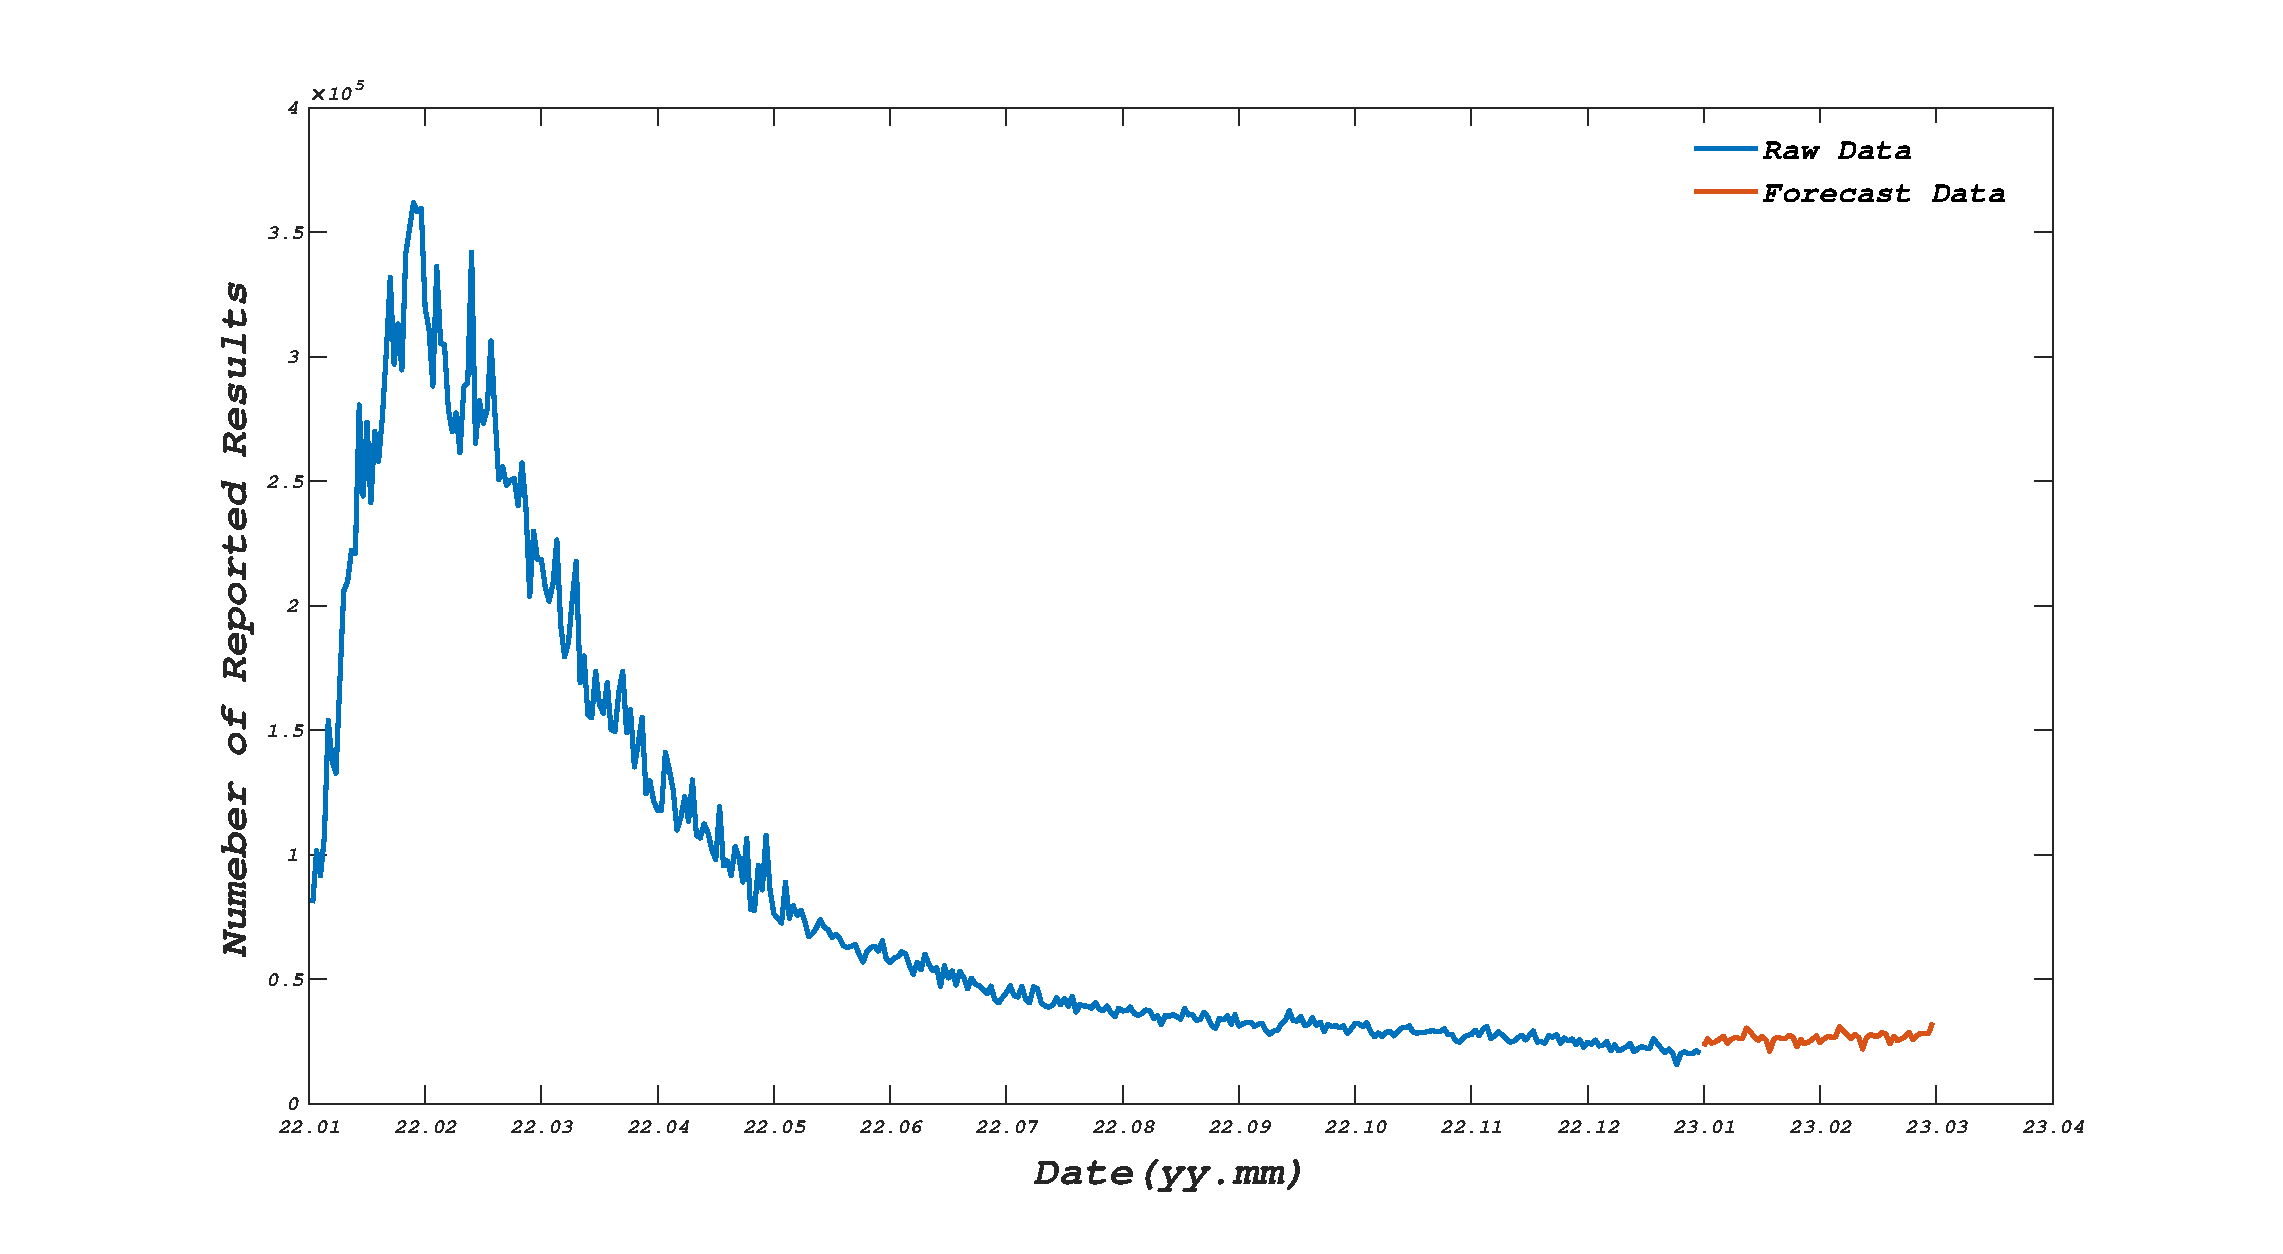
\includegraphics[width=\textwidth]{img/yuce.eps}\caption{Prediction Results}
% \end{subfigure}
% \begin{subfigure}[b]{.49\textwidth}
% 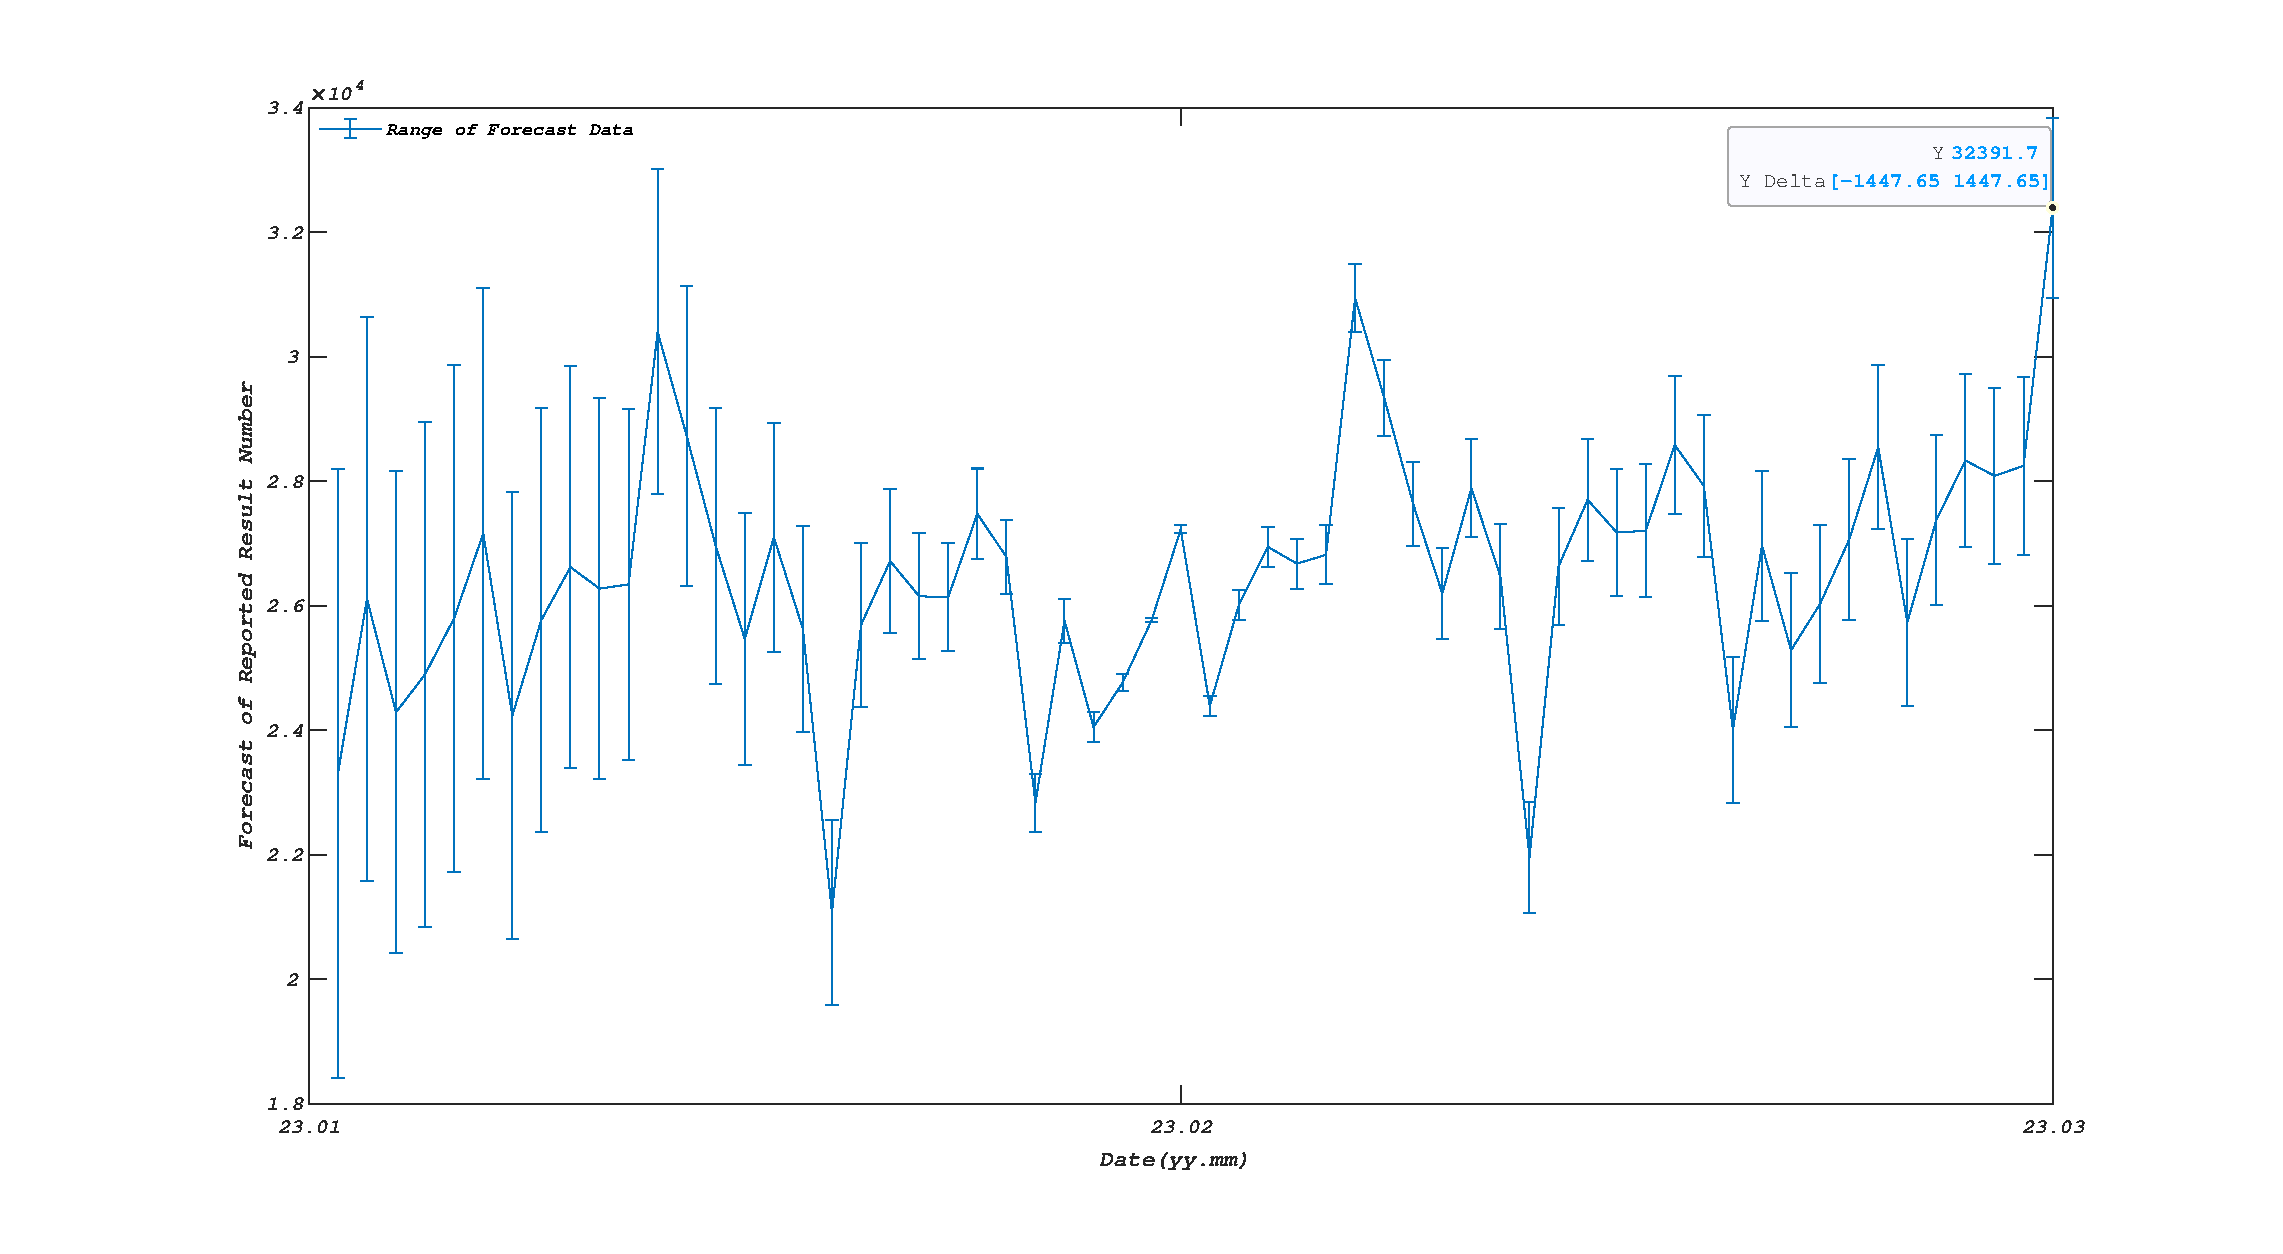
\includegraphics[width=\textwidth]{img/wucha.eps}\caption{Prediction Interval}
% \end{subfigure}
% \caption{ARIMA(5,1,2) Model Predict}
% \end{figure}
\begin{figure}[htbp]
\centering
\begin{subfigure}[b]{.49\textwidth}
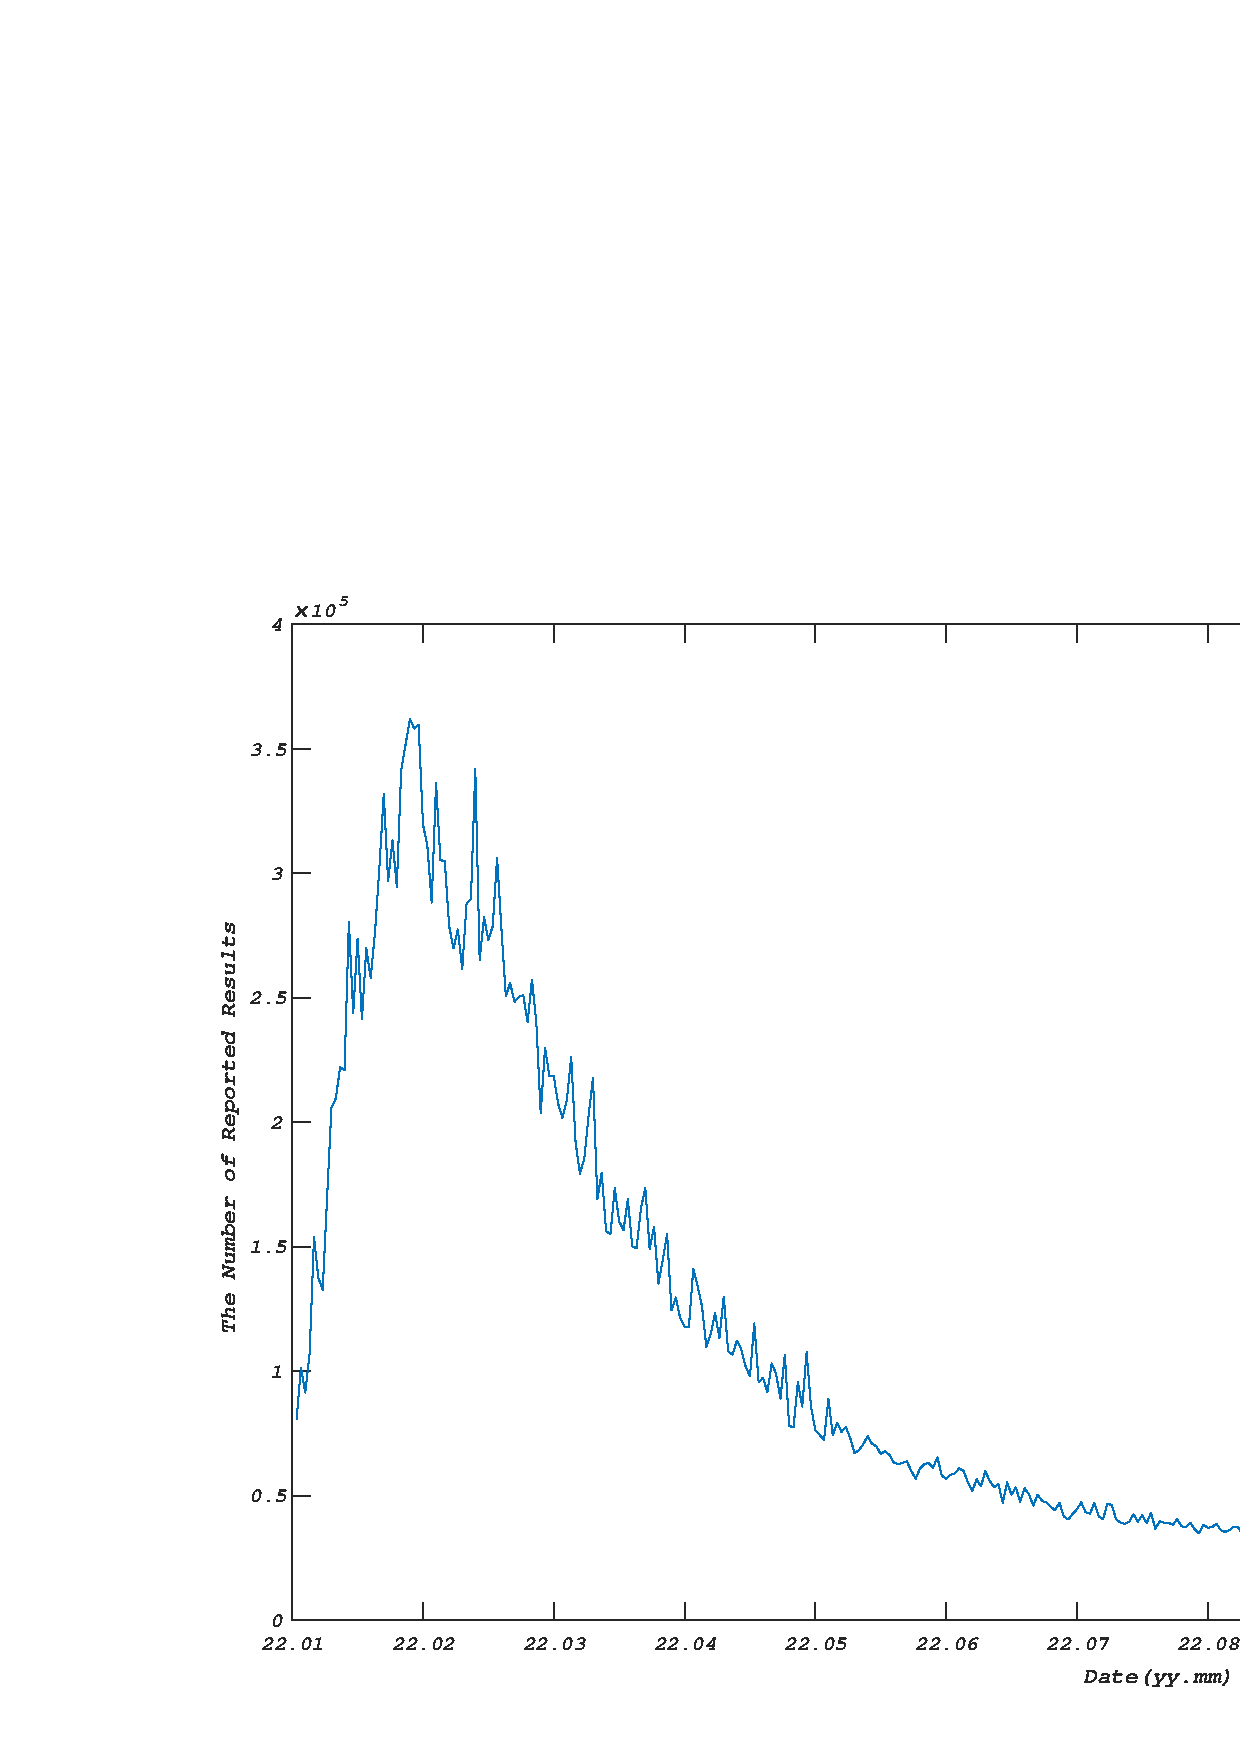
\includegraphics[width=\textwidth]{img/yuanshi.pdf}\caption{Prediction Results}
\end{subfigure}
\begin{subfigure}[b]{.49\textwidth}
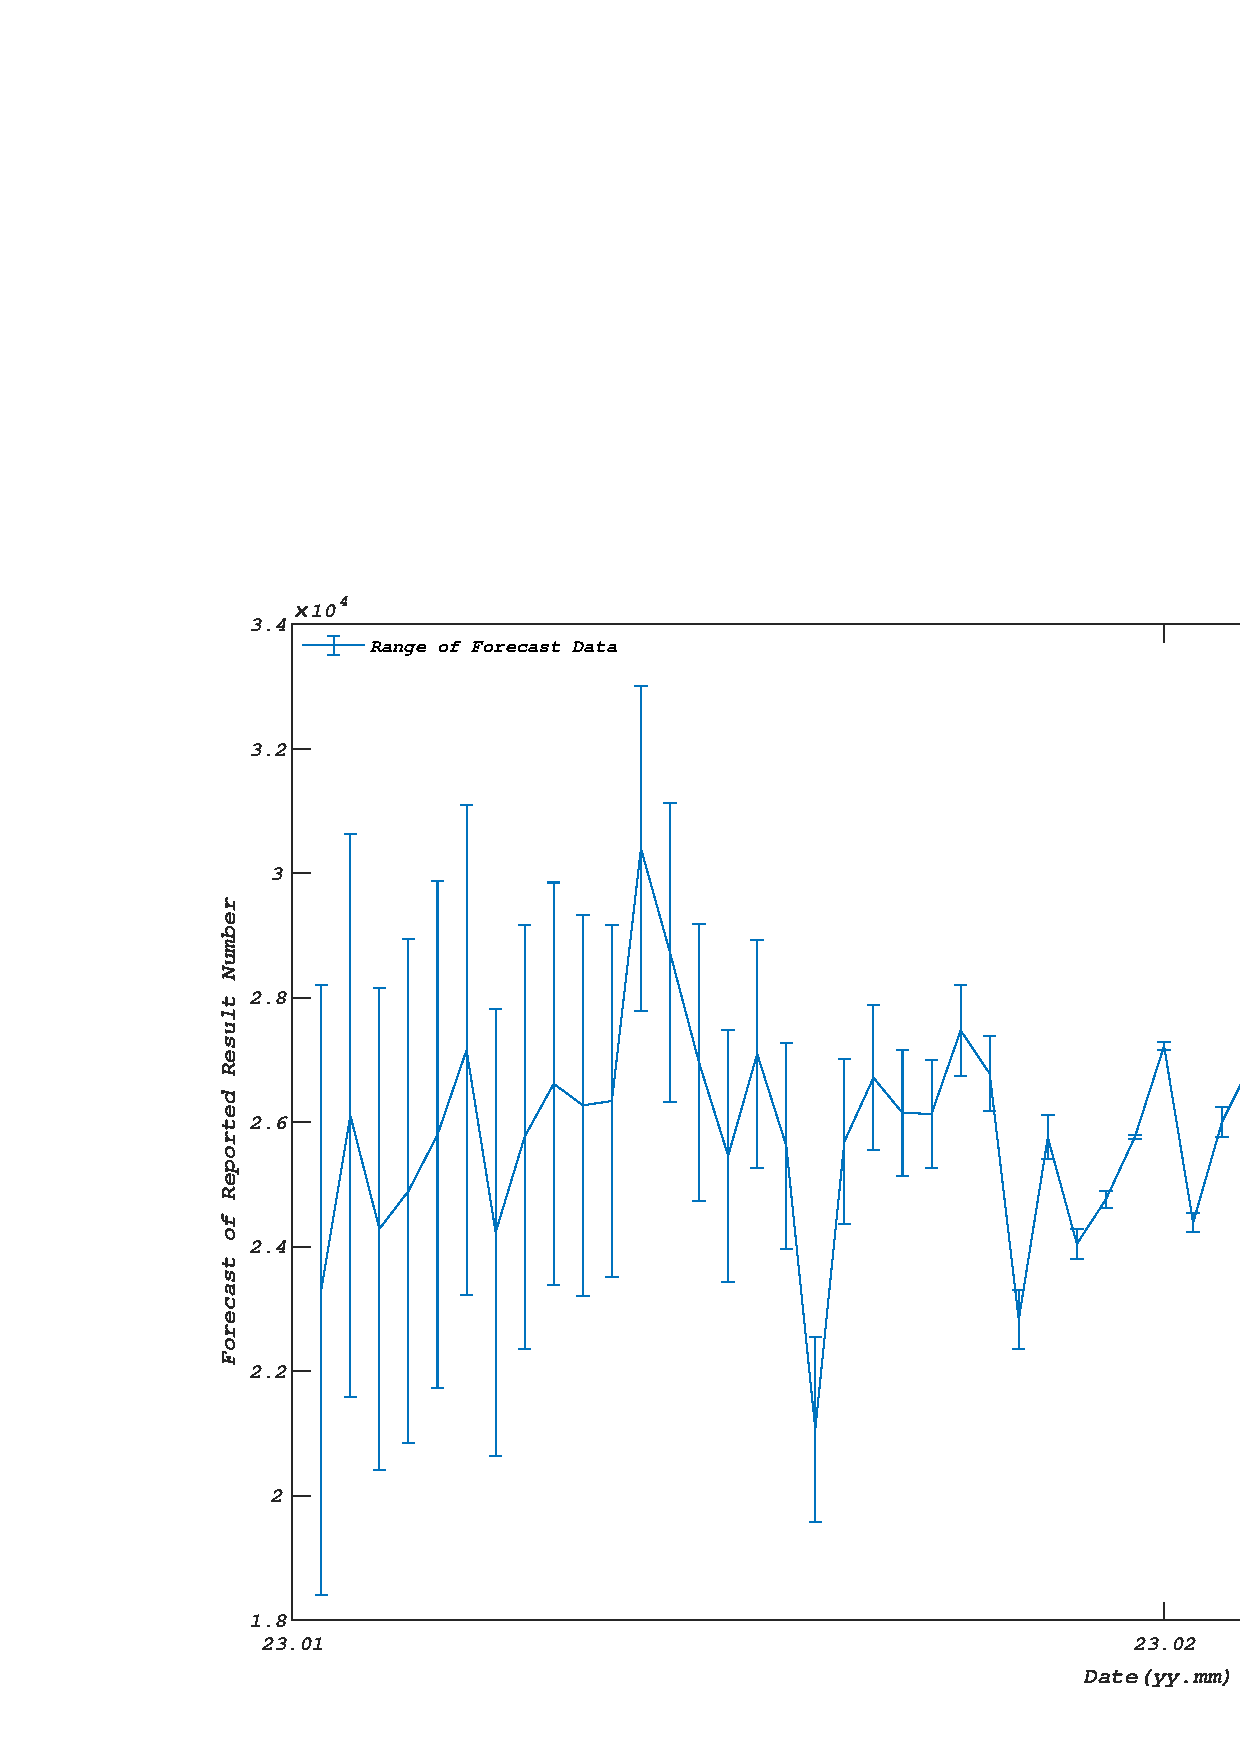
\includegraphics[width=\textwidth]{img/wucha.pdf}\caption{Prediction Interval}
\end{subfigure}
\caption{ARIMA(5,1,2) Model Predict}
\end{figure}
\subsection{Establishment of LSTM-ARIMA Model}
\subsubsection{Improved ARIMA model: LSTM-ARIMA Model}
For the ARIMA model, the precision of prediction is limited, and the fitting and prediction results are not optimistic when the data have strong volatility. However, the Long Short Term Memory (\textbf{LSTM}) model does not have high requirement for data, however, because of the small amount of data, we can not give a good forecast, so we combine the advantages of the two, to improve the ARIMA model established LSTM-ARIMA model.
\subsubsection{Workflow of Hybrid LSTM-ARIMA Model}
The LSTM-ARIMA model works as shown in the Figure \ref{yuanli}:
\begin{figure}[htbp]
\centering
\includegraphics[width=\textwidth]{img/document1.pdf}
\caption{Workflow of Hybrid LSTM-ARIMA Model}\label{yuanli}
\end{figure}
\subsubsection{Data Predictions Using LSTM-ARIMA Model}
Predictions are produced through the execution of appropriate algorithms in this stage. In the following paper, the two algorithms are combined to predict results, LSTM (long-term memory) and others are ARIMA (Auto Regressive Integrated Moving Average). Both algorithms represent distinct forecast. And the outcome was acquired in the form of RMSE and MAPE values.

In LSTM process the output of one node is given as a input to the another state. The updating of new state takes place in the form given in Equation \ref{gongshi1}:
\begin{eqnarray}
B_v=f_v\cdot B_{v-1}+i_v\cdot B_v'\label{gongshi1} 
\end{eqnarray}
Where, $B_v$ refers to new state or updated state, $f_v$ refers to function value, $B_{v-1}$ refers to old state, $i_v$ refers to input value, $B_v'$ refers to candidate value.
\subsubsection{Hybrid LSTM-ARIMA Algorithm}
Here we use the LSTM-ARIMA model to fit and predict the percentage of different attempts in the future, which requires less data and is able to obtain more accurate results, and the algorithm is shown below:
\begin{algorithm}
\caption{Hybrid LSTM-ARIMA Algorithm}
Data sets,
Read the files,
Train the data file\;
Model=sequential\;
\quad Model.add LSTM (units= 100)\;
\quad Model.add Dense (1) where activation=``double-tanh''\;
\quad Model.add Flatten\;
Repeat the process\;
\quad Do the forward-propagation model with train-X\;
\quad Do the backward-propagation model with train-Y\;
\quad Refurnished or updation of parameters of model\;
\quad In all Time series $T_i$ in data do\;
Model=NULL\;
For all order in orders do\;
\quad Rorder = For ARIMA [$T_i$, order]\;
\quad Add Rorder to models\;
Unused = X – predict ($T_i$, $R_{fit}$)\;
\quad Add unused to X\;
\quad Add unused to Y\;
\quad Reserve save X and Y\;
Train-RMSE, Train-MAPE = model (train-X, train-Y).\;
\quad Calculate dev-RMSE, dev-MAPE = model (dev-X, dev-Y)\;
End repeat\;
Test-RMSE, test-MAPE = model (test-X, test-Y)\;
END
\end{algorithm}
\subsubsection{Comparison of RSEM Values with ARIMA Model}
The RMSE values show that when LSTM is mixed with the ARIMA model, it acquires the characteristics of both techniques, and the results obtained show the best accuracy compared to other models.We list their RMSE values in Table \ref {rmse}:
\begin{table}[!h]
\begin{center}
\caption{Comparison of RSEM Value}\label{rmse}
\begin{tabular}{cc}
	\hline
\textbf{Model} & \textbf{RMSE Value}                                           \\ \hline
LSTM-ARIMA          & 7.254823                                                         \\
ARIMA     & 8.884206 \\ \hline
\end{tabular}
\end{center}
\end{table}
\subsection{Prediction with LSTM-ARIMA Model}
Here we use our trained LSTM-ARIMA model to predict the percentage of different attempts in the future. In order to compare with the ARIMA model, we will predict the number of different attempts in the future (which invariably puts a huge pressure on our model), and then make a comparative analysis with the ARIMA model predictions. We give the predicted percentage of each attempt in the form of a heat map and also gave a predicted distribution of \textbf{the number of solutions for the word ``EERIE'' on 2023 March 1 as} \bm{$(1,2,3,4,5,6, X) = (1,21,12,14,30,18,4)$}.
\begin{figure}[htpb]
\centering
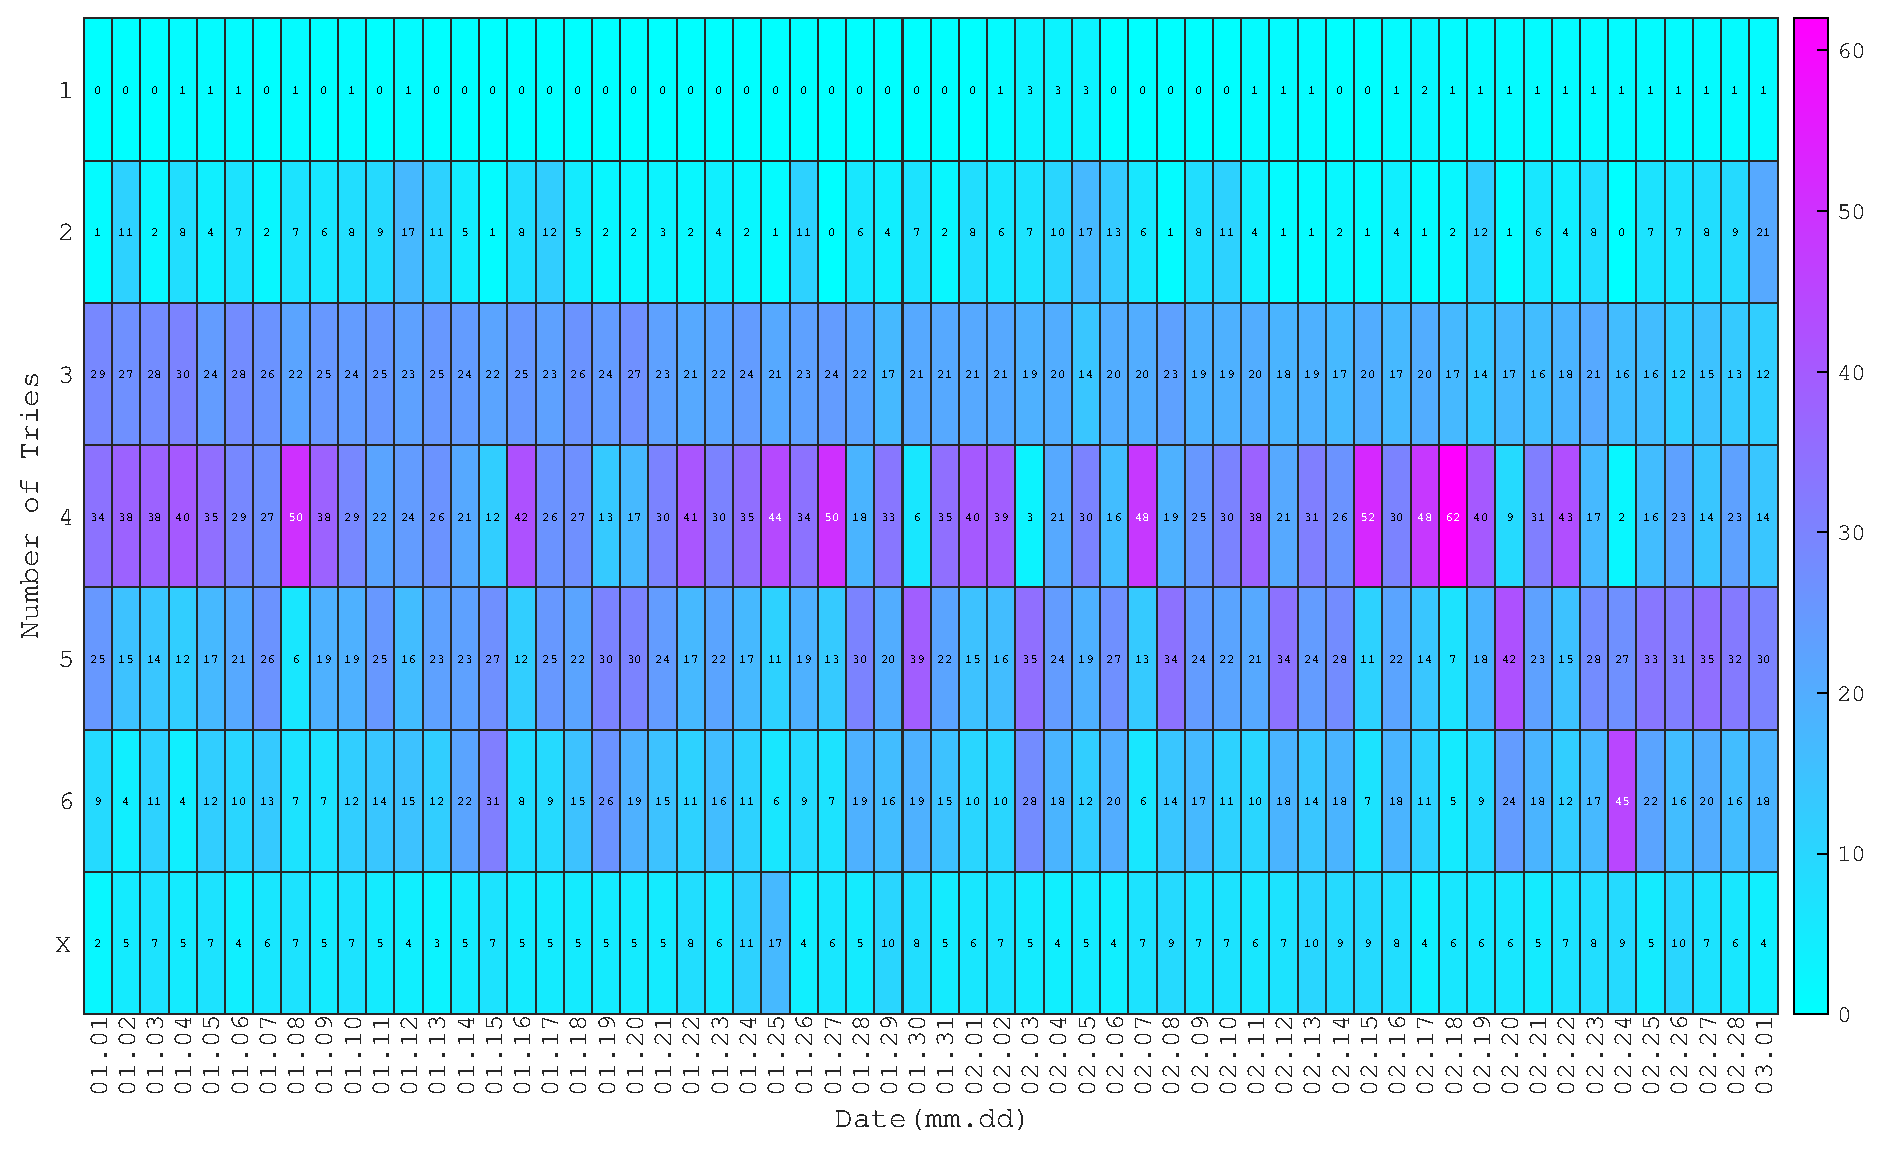
\includegraphics[width=.8\textwidth]{img/hmap.eps}
\caption{Prediction of Tries Number}
\end{figure}
\begin{figure}[htbp]
\centering
\includegraphics[width=.95\textwidth]{img/lstm.pdf}
\caption{Model Prediction Comparison}
\end{figure}













\newpage
\section{{\sc \textbf{Task 2}}: Discussion of Words}
% \subsection{Percentage of Difficult Mode}
% To find out whether the properties of the word itself affect the percentage of people playing in difficult mode, we first assume that there is no correlation between the two. We plot the percentage of people playing in difficult mode versus time, and to show this percentage more visually over time, we fit a cubic polynomial to it and shown that in Figure \ref{sancinihe}:
% \begin{figure}[htbp]
% \centering
% 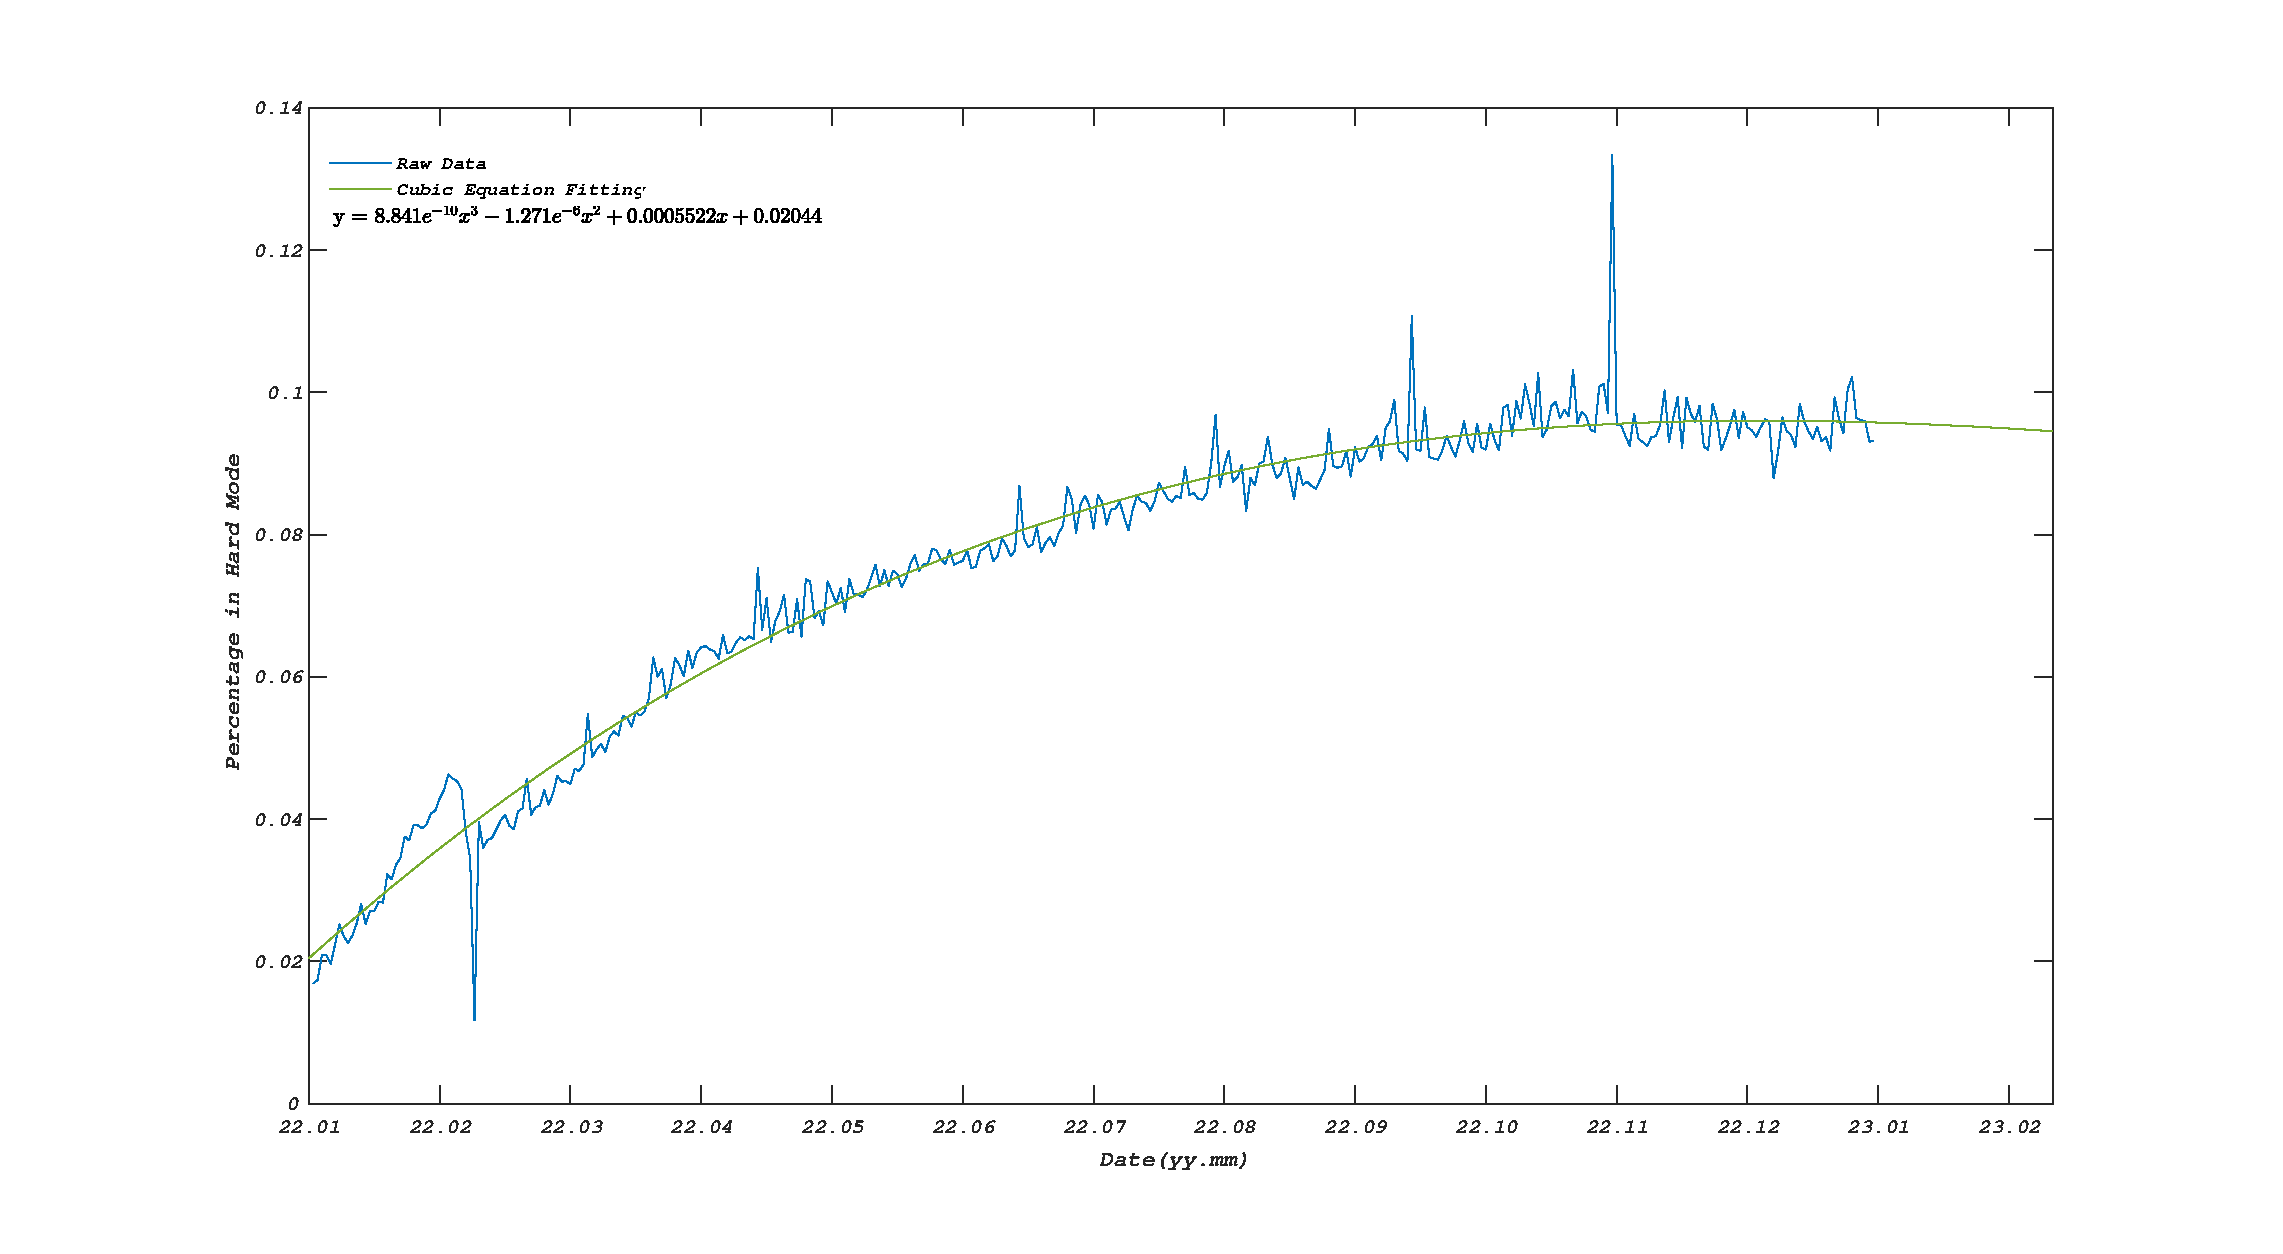
\includegraphics[width=\textwidth]{img/sanci.eps}
% \caption{Cubic Polynomial Fitting}\label{sancinihe}
% \end{figure}

% We found that the percentage of people playing in the difficult mode basically obeyed the distribution of the cubic polynomial $y=8.841e^{-10}x^3-1.271e^{-6}x^2+0.0005522x+0.02044$($R^2$ reached 0.9681, and the Residual Norm was only 0.07525), and the words were given completely randomly, not with We therefore believe that the percentage of people playing the game in difficult mode is not related to the nature of the words themselves. The reason for this is that we are not told in advance that the word is more difficult and we are advised not to enable hard mode or we are told that the word is easier and we are forced to open hard mode in order to increase the playability of the game: this is certainly not possible. We would venture to guess that the increase in the number of people choosing to play in hard mode is due to the increased popularity of the game and the fact that they are actively choosing hard mode in order to be able to ``show off'' their ``battle results'' on Twitter (Of course, this is just our guess, the actual situation may be very complicated, in fact, people's thoughts cannot be completely unified).
\subsection{The Nature of The Word Itself}
We studied the properties of the words themselves and found the following factors influencing word difficulty with limited data support.
\begin{itemize}
\item Number of words
\item Word Types
\item Number of letters contained in the word (repeated letters are not counted repeatedly, if they contain repeated letters, they are counted only once)
\item The alphabetic heat of the word (the percentage of occurrences of each letter contained in the calendar)
\item Number of word meanings
\end{itemize}
Our processing steps for the indicators are as follows.
\begin{enumerate}[Step 1]
\item We pre-processed the data to remove some of the problematic data (e.g. words containing only four letters)
\item The rate of appearance of each letter, the proportion of the number of successful guesses to the total number of reports per day, and the average number of guesses used per day were calculated
\item The average number of unduplicated letters is assigned:
\begin{itemize}
\item Words containing both verb and noun morphemes are worth 1 points.
\item Words with a verb or noun part of speech are worth 2 points.
\item Words that contain neither verbal nor noun lexemes are worth 3 points.
\end{itemize}
\item We then stratified these data to obtain the Table \ref{tf}.
\end{enumerate}
\begin{table}
\centering\caption{Factors That Affect The Difficulty of Words}\label{tf}
\includegraphics[width=\textwidth]{img/工作簿1.pdf}
\end{table}





\subsection{Establishment of AHP-EWM-TOPSIS Model}
\subsubsection{EWM for Obtaining Weight Coefficients}
Entropy Weight Method(\textbf{EWM}) is an objective weighting method obtained from the characteristics of decision matrix data, which makes full use of the structural information of the decision matrix to analyze the weight coefficients of each objective, and is applicable to the situation where there is little or no correlation between evaluation objects.
Calculating the entropy $E_j$ from the decision matrix $B$, we have:
\begin{eqnarray}
E_j=-K\sum_{j=1}^{m}\frac{x_{ij}}{e_{ij}}\ln(\frac{x_{ij}}{e_{ij}})
\end{eqnarray}
\begin{eqnarray}
e_{ij}=\sum_{i=1}^{m}x_{ij}
\end{eqnarray}
Where, $i=1,2,\cdots,m,j=1,2,\cdots ,n$,$K$ refers to the constant coefficient, $x_{ij}$ is the value of the $j$-th evaluation index of the $i$-th program, $ E_j$ is the entropy value of the $j$-th index, and thereinto, $E_j\in [0,1]$.

Define $f_j$ as the degree of consistency in the contribution of each program under the $j$-th evaluation metric, we have:
\begin{eqnarray}
\theta _j=\frac{f_i}{\sum_{j=1}^{n}f_j}
\end{eqnarray}

It can be seen that when the values of a certain evaluation indicator converge among the programs, $f_j$ tends to 0, which indicates that there is no difference among the programs for that evaluation indicator, the influence of that evaluation indicator on the evaluation contribution of the program is small, and the value of the weight coefficient of that evaluation indicator is small; when the values of a certain evaluation indicator differ significantly among the programs, $f_j$tends to 1, which indicates that the influence of that evaluation indicator on the evaluation contribution of the program is large, and the value of the weight coefficient of that evaluation indicator is large.
\subsubsection{AHP-EWM Weight calculation}
In order to combine the weights obtained by subjective and objective weighting methods, and considering the different dispersion of different index values, the fixed weight preference coefficients cannot fully reflect the information characteristics of EWM, the final index weights are obtained by using the distance index $\rho _j$ as the composite weight.

Combining the derived Analytic Hierarchy Process(\textbf{AHP}) weight coefficients $\omega _j$ and EWM weight coefficients $\theta _j$, the composite weight $\rho_j$ can be expressed as Equation \ref{rj}:
\begin{eqnarray}
\rho _j=\sqrt{(\varepsilon _j\omega _j)^2+[(1-\varepsilon _j)\theta _j]^2}\label{rj}
\end{eqnarray}

To determine the value of $\varepsilon_j$, a planning model can be built using the least squares method with Equation \ref{with}:
\begin{eqnarray}
\min\rho _j=\sqrt{(\varepsilon _j\omega _j)^2+[(1-\varepsilon _j)\theta _j]^2} \ \  s.t. 0\le \varepsilon \le 1
\label{with}
\end{eqnarray}

The dynamic weight preference coefficient $\varepsilon _j$ is obtained by solving for:
\begin{eqnarray}
\varepsilon _j=\frac{\theta _j^2}{\omega _j^2+\theta _j^2} 
\end{eqnarray}




























\subsubsection{AHP-EWM-TOPSIS Comprehensive Evaluation Model}
The basic principle of Technique for Order Preference by Similarity to Ideal Solution(\textbf{TOPSIS}) is to rank the solutions to be evaluated by the relative distance between the positive and negative ideal solutions of a multi-objective decision problem. The positive ideal solution is usually the fictitious best solution, and each indicator is the best value of the solution to be evaluated; the negative ideal solution is the worst value of the solution to be evaluated, and TOPSIS ranks the solutions in a comprehensive manner by considering the convergence of the solutions to the positive and negative ideal solutions.

Obviously, the closer the solution is to the positive ideal solution, the better the solution is.
\begin{enumerate}
    \renewcommand{\labelenumi}{\textbf{Step \theenumi}}
\item Initialization of judgment matrix

$U=\{U_1,U_2,\cdots ,U_m\}$ is the set of scenarios, where $U_i(0\le i\le m)$ is the $i$-th feasible scenario, and the set of evaluation indicators for each scenario is set to $P=\{P_1,P_2,\cdots ,P_n\}$, with $x_{ij}(0<i\le m,0<j\le n)$ denoting the $j$-th evaluation indicator value of the $i$-th scenario, a decision matrix $B$ can be built as:
\begin{eqnarray}
B=(x_{ij})_{m\times n}=\begin{bmatrix}
 x_{11} & x_{12} &\cdots& x_{1n}\\
 x_{21} &x_{22}  &\cdots  &x_{2n} \\
  \vdots &\vdots   & \ddots  & \vdots \\
 x_{m1} &x_{m2}  &\cdots  &x_{mn}
\end{bmatrix}_{m\times n}
\end{eqnarray}
\item Normalizing the evaluation metrics:
\begin{eqnarray}
r_{ij}={x_{ij}}/{\max_{j}x_{ij}}
\end{eqnarray}
\begin{eqnarray}
r_{ij}'=\frac{r_{ij}}{\sum_{i=1}^{m}r_{ij}}
\end{eqnarray}
\item Obtained the final normalized decision matrix:
\begin{eqnarray}
R=(r_{ij}')_{m\times n}=\begin{bmatrix}
 r_{11}' & r_{12}' &\cdots& r_{1n}'\\
 r_{21}' &r_{22}'  &\cdots  &r_{2n}' \\
  \vdots &\vdots   & \ddots  & \vdots \\
 r_{m1}' &r_{m2}'  &\cdots  &r_{mn}'
\end{bmatrix}_{m\times n}
\end{eqnarray}
\item Define maximum and minimum values:
\begin{eqnarray}
Z^+=(Z_1^+,Z_2^+,\cdots,Z_m^+)
\end{eqnarray}
\begin{eqnarray}
Z^-=(Z_1^-,Z_2^-,\cdots,Z_m^-)
\end{eqnarray}
Where, $Z_k^+=\max\{z_{1k},z_{2k},\cdots ,z_{nk}\}$, $Z_k^-=\max\{z_{1k},z_{2k},\cdots ,z_{nk}\}$
\item Define the distance of the $i$-th evaluation object from the maximum and minimum values:
\begin{eqnarray}
D_i^+=\sqrt{\sum_{j=1}^{m}(Z_j^+-z_{ij})^2}
\end{eqnarray}
\begin{eqnarray}
D_i^-=\sqrt{\sum_{j=1}^{m}(Z_j^--z_{ij})^2}
\end{eqnarray}
\item Calculate the unnormalized score:
\begin{eqnarray}
Score_i=\frac{D_i^-}{D_i^++D_i^-}
\end{eqnarray}
\end{enumerate}
\subsection{Solution of AHP-EWM-TOPSIS Model}
We scored 355 evaluation objects (there were 4 anomalous words and we did not score them) by the model we built and classified the difficulty levels as follows:
\begin{table}[!h]
\begin{center}
\caption{Accuracy of Our Model}\label{acc}
\begin{tabular}{cc}
\hline
Score&Levels\\\hline
$Under$ 5.15&Entry Level\\
$5.15-5.65$&Intermediate Level\\
$5.65-6.15$&Advanced Level\\
$6.15-6.65$&Hard Level\\
$Above$ 6.65&Hell Level\\\hline
\end{tabular}
\end{center}
\end{table}

Next, we scored the word ``EERIE'' and determined its corresponding difficulty: we scored the word ``EERIE'' with a score of 7.135, which corresponds to the above difficulty level of hell level. ``EERIE'' consists of three non-repeating letters ``E'', ``R'', and ``I'', of which ``E'' appears three times, which is a bit difficult to think of, but ``E'' and ``R'' are in the top three of all words that have ever appeared. This reduces the difficulty of ``EERIE'' to some extent, but it is so insignificant for the hellish ``EERIE'' because ``EERIE'' has one and only one adjective, and contains only four meanings, among which there are Two of them only appear in a very few dictionaries and on the Internet, and it means ``suggestive of the supernatural'', and people rarely use it, and when they do, they choose more common words like terrible or fearful, so people have a hard time thinking about it.

At the same time, in order to reduce the error as much as possible, we use the multiple linear regression model to test the correlation of the factors that may affect the difficulty of words. The fitting results show that the part of speech, the meaning, the number of non-repeating letters and the proportion of letters appearing are all related to the difficulty of words, among which the number of word meanings is the highest fitting, which is the same as the factor with the highest weight obtained by our model.
\subsection{Same Characteristics for Different Difficulty Levels.}
\begin{itemize}
	\item Entry Level
\end{itemize}
The difficulty of the words is below 5.15 points, and the average number of successful uses is about 3.31. Most of the words have both verbal and noun words, and the words are more commonly used in people's lives, and it is easier for people to remember the words with the same meaning and have a variety of words and meanings.
\begin{itemize}
	\item Intermediate Level
\end{itemize}
The difficulty of the words ranged from 5.15 to 5.65, and the average number of successful uses of about 3.87, with at least one of the verb and noun conjugations, and words that are so common that most people learning English but not native speakers can recognize most of them.
\begin{itemize}
	\item Advanced Level
\end{itemize}
The difficulty of the words ranged from 5.65 to 6.15, and the average number of successful uses is about 4.14, which is difficult, but not very difficult, and most of them contain two or more meanings that are not close to each other
\begin{itemize}
	\item Hard Level
\end{itemize}
The difficulty of the words ranged from 6.15 to 6.65 points, and the average number of successful uses was about 4.20. Most of the words were less commonly used, and their meanings may be modifiers of infrequently used items or words depicting particular circumstances.
\begin{itemize}
	\item Hell Level
\end{itemize}
The difficulty of the words is above 6.65, and the average number of successful uses is about 4.81. Most of the words have a single meaning, and the combination of letters is peculiar, such as "EERIE" has three numbers of E, and its near-synonyms are easier to remember than the original words.
















































































\section{{\sc \textbf{Task 3}}: Evaluation of Our Model}
\subsection{Evaluation of ARIMA \& LSTM-ARIMA Model}
In order to evaluate the confidence of the model, we first define the prediction accuracy number $T$ in the test set: when the error between the prediction result and the actual result does not exceed 1\% (here because we need rounding for the percentage of word guesses, if the error does not exceed 1\%, then the rounded percentage we think should still be the same. That is, in the prediction of the percentage of word guesses, we think that the error of 1\% does not affect the prediction of the model), and we think its prediction is accurate. Next, we adopt \textbf{Accuracy} as the evaluation index to evaluate the confidence level of the model. The following gives their calculation Equation \ref{tn}:
\begin{eqnarray}
Accuracy=\frac{T}{N}\label{tn}
\end{eqnarray}
Where, $N$ refers to the number of samples in the test set. The larger the value of Accuracy, the better the model performance. Here we list the Accuracy of our model in the following table:
\begin{table}[!h]
\begin{center}
\caption{Accuracy of Our Model}\label{acc}
\begin{tabular}{cc}
\hline
\textbf{Model}&\textbf{Accuracy(\%)}\\ \hline
ARIMA&84.46\\
LSTM-ARIMA&93.37\\\hline
\end{tabular}
\end{center}
\end{table}

From Table \ref{acc}, we can see that the accuracy of ARIMA model is 84.46\%, while the accuracy of LSTM-ARIMA model is 93.37\%. So it seems that the prediction effect of ARIMA(5,1,2) model we started to establish is not very good. Of course, if we add errors to make interval prediction, the accuracy of ARIMA(5,1,2) model should be higher. The accuracy of LSTM-ARIMA model is 93.37\% with an error of 1\%. \textbf{Therefore, we have 93.37\% confidence in the model to predict the proportion of word guessing times is accurate}.


\subsection{Evaluation of AHP-EWM-TOPSIS Model}
In the solution of the AHP-EWM-TOPSIS model, we obtained the difficulty score of each word. In order to evaluate the accuracy of this prediction model, we consider the actual difficulty of the words to be related to the proportion of words guessed in that day's game, and we directly weight the number of correct guesses for each: if you guess the word on the first time, then congratulations, you get 6 points, but if you guess it on the sixth time, then unfortunately, you can only get one point. So the score vector for the number of times you guessed the word while playing the game is given as follows:
\begin{eqnarray}
SETT=[S_1,S_2,S_3,S_4,S_5,S_6,S_X]=[6,5,4,3,2,1,0]
\end{eqnarray}
Where, $SETT$ refers to Scores of Each Try Times, $S_k(k=1,2,\cdots,6)$ refers toScore for the number of words guessed at the $k$-th time(Scores of $k$-th Tries), $S_X$ refers to the score for not guessing the word in six chances is 0.

% We calculate the total score based on the percentage of each number of times the word was guessed each day(PENTG)multiplied by the score as follows.
\begin{enumerate}
    \renewcommand{\labelenumi}{\textbf{Step \theenumi}}
\item We calculate the total score based on the percentage of each number of times the word was guessed each day(\textbf{PENTG})multiplied by the score as follows.
\begin{eqnarray}
PENTG=[p_1,p_2,p_3,p_4,p_5,p_6,p_X]
\end{eqnarray}
\begin{eqnarray}
Score’=SETT\times PENTG 
\end{eqnarray}
Where, $p_k(k=1,2,\cdots,6)$ refers to the percentage of words guessed at the $k$-th, $p_X$ refers to the percentage of words that were not guessed within six times.
\item To eliminate the effect of score differences, we need to normalize both $Score$ and $score'$ so that the scores fall in the $[0,1]$ range:
\begin{eqnarray}
N_{Score}=\frac{Score-\min(Score)}{\max(Score)-\min(Score)}
\end{eqnarray}
\begin{eqnarray}
N_{Score}'=\frac{Score'-\min(Score')}{\max(Score')-\min(Score')}
\end{eqnarray}
Where, $N_{Score}$ refers to the scores of the AHP-EWM-TOPSIS Model after normalization of the scores of, $N_{Score}'$ refers to the scores normalized under SETT and PENTG. 
\item The relative error between $N_{Score}$ and $N_{Score}'$ is then calculated as follows:
\begin{eqnarray}
\delta =\frac{\Delta}{L}\times 100\%=\frac{N_{Score}-N_{Score}'}{N_{Score}'}\times 100\%
\end{eqnarray}
Where, $\delta$ refers to actual relative error, $\Delta$ refers to absolute error, here $L=N_{Score}'$.
\item Calculate the value of Accuracy.
\begin{eqnarray}
Accuracy=1-\mathrm{Average}(|\delta|)
\end{eqnarray}
\end{enumerate}
\textbf{We obtained the Accuracy as 79.603\%} and we show the $\delta$ value in the Figure \ref{delta}:
\begin{figure}[htbp]
\centering
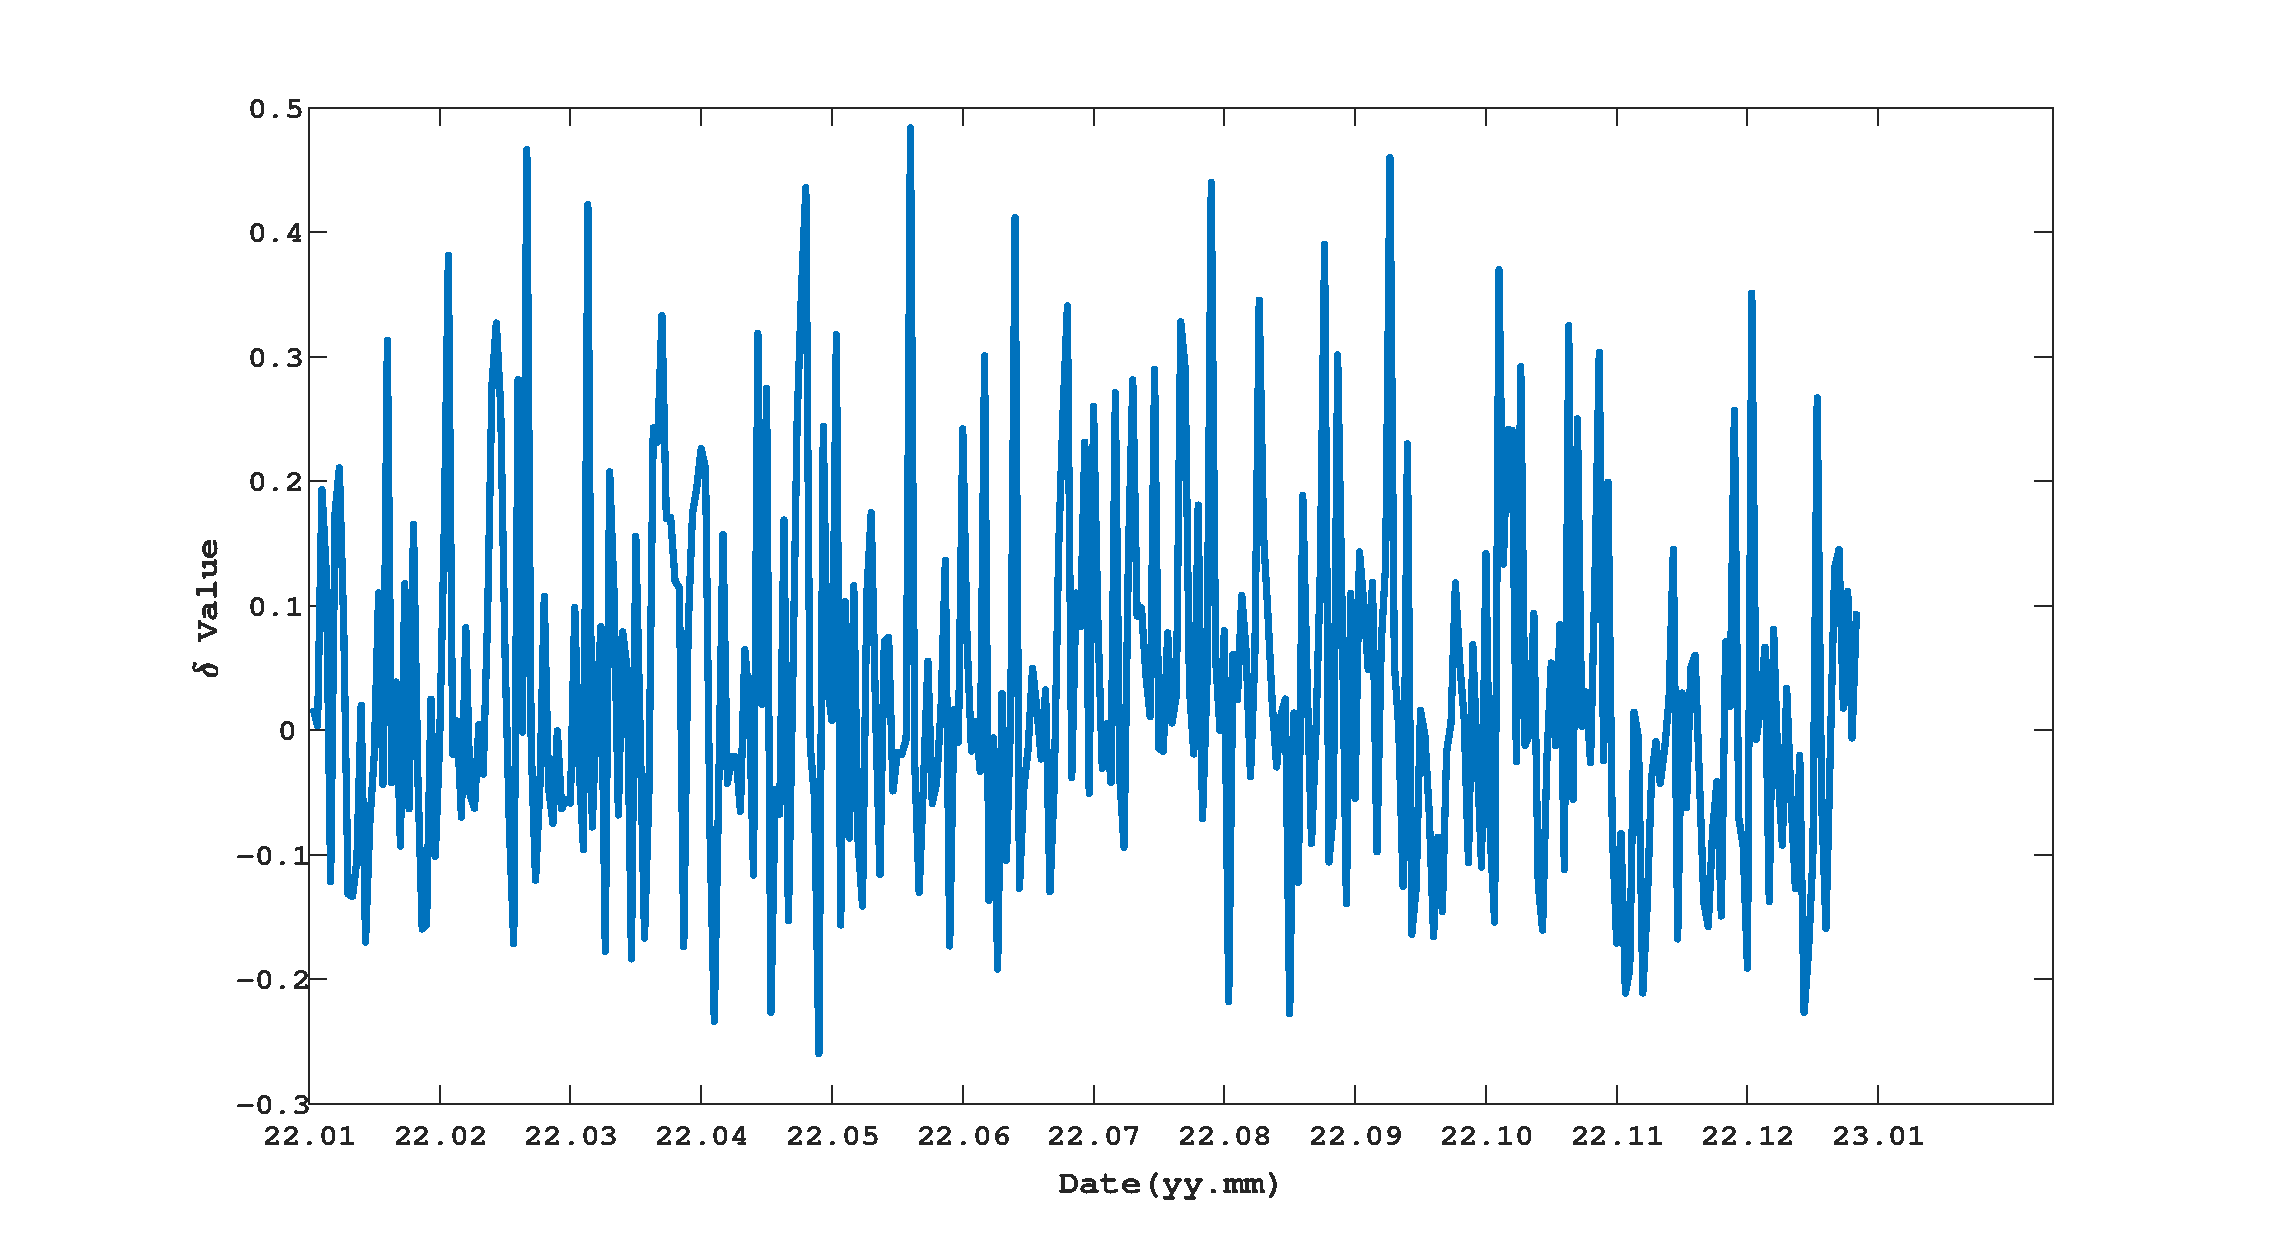
\includegraphics[width=\textwidth]{img/delta.eps}
\caption{The $\delta$ Value of Our Model}\label{delta}
\end{figure}











% \subsection{Strengths and Weaknesses}
% Our research is basically based on the predecessors, and there are some improvements and shortcomings as follows:
% \subsubsection{Strengths}
% \subsubsection{Weaknesses}
% \subsection{Future Work}























































% The instance of long and wide tables are shown in Table \ref{tb:longtable}.

% % 长表格示例,更多用法请参考 longtable 宏包文档
% % 以下环境及对应参数可实现表格内的自动换行与表格的自动断页
% % 您也可以选择自行载入 tabularx 宏包,并通过 X 参数指定对应列自动换行
% \begin{longtable}{ p{4em} p{14em} p{14em} }
% \caption{Basic Information about Three Main Continents (scratched from Wikipedia)}
% \label{tb:longtable}\\
% \toprule
% Continent & Description & Information \\
% \midrule
% Africa & Africa Continent is surrounded by the Mediterranean Sea to the
% north, the Isthmus of Suez and the Red Sea to the northeast, the Indian
% Ocean to the southeast and the Atlantic Ocean to the west. &
% At about 30.3 million km$^2$ including adjacent islands, it covers 6\%
% of Earth's total surface area and 20\% of its land area. With 1.3
% billion people as of 2018, it accounts for about 16\% of the world's
% human population. \\
% \midrule
% Asia & Asia is Earth's largest and most populous continent which
% located primarily in the Eastern and Northern Hemispheres.
% It shares the continental landmass of Eurasia with the continent
% of Europe and the continental landmass of Afro-Eurasia with both
% Europe and Africa. &
% Asia covers an area of 44,579,000 square kilometres, about 30\%
% of Earth's total land area and 8.7\% of the Earth's total surface
% area. Its 4.5 billion people (as of June 2019) constitute roughly
% 60\% of the world's population. \\
% \midrule
% Europe & Europe is a continent located entirely in the Northern
% Hemisphere and mostly in the Eastern Hemisphere. It comprises the
% westernmost part of Eurasia and is bordered by the Arctic Ocean to
% the north, the Atlantic Ocean to the west, the Mediterranean Sea to
% the south, and Asia to the east. &
% Europe covers about 10,180,000 km$^2$, or 2\% of the Earth's surface
% (6.8\% of land area), making it the second smallest
% continent. Europe had a total population of about 741 million (about
% 11\% of the world population) as of 2018. \\
% \bottomrule
% \end{longtable}















\section{Some Other Interesting Properties}
In our dataset, we have calculated the number of people who successfully guessed the word and their proportion, and found that on average, 97.1775\% of people can complete the guessing. However, in real life, it doesn't seem to be the case (at least our team found it difficult to guarantee not to use external help to guess), and because there are many rare words in the game, we can almost certainly say that there is an important factor leading to the success rate of the game exceeding the real value. We noticed the source of the data: Twitter! This can be easily explained: because of self-esteem, more people are not willing to share their failures, so successful examples on Twitter are always much more than failed ones, which explains why the success rate in the data is so high.

We have counted the occurrence and frequency of all the letters in the dataset and found that the five letters with the highest frequency are `e', `a', `r', `o', and `t'. Therefore, we have reason to believe that if a five-letter word consists of these letters arranged in this specific order, it should be the easiest to guess (you are more likely to get green and yellow tiles than gray ones). Based on this, we have identified three possible words: ``oater'', ``orate'' and ``roate''.

Upon further observation of the statistical results, we found that the letter `e', which ranked first in frequency, appeared 46 times more often than the letter `j', which ranked last in frequency. This is quite reasonable as vowels generally have a higher frequency of occurrence. However, it is possible that the high frequency of these letters is due to an overinterpretation caused by a small sample size (although in fact, this is consistent with the ranking given by Google).
\begin{figure}[htbp]
\centering
\includegraphics[width=\textwidth]{img/zimu.pdf}
\caption{Frequency of letters}
\end{figure}


% 以下为信件/备忘录部分,不需要可自行去掉
% 如有需要可将整个 letter 环境移动到文章开头或中间
% 请在第二个花括号内填写标题,如「信件」(Letter)或「备忘录」(Memorandum)
\begin{letter}{Letter}
\begin{flushleft}  % 左对齐环境,无首行缩进
\textbf{To:} MCM/ICM organizing committee\\
\textbf{From:} Team \# 231846\\
\textbf{Date:} \today\\
\textbf{Dear Puzzle Editor of the New York Times: }
\end{flushleft}
\lettrine{H}{ere} our team will report to you our team's research and findings, and give you some of our team's recommendations on ``WORDLE'' game, please check out:
{\large{\itshape \begin{enumerate}[0]
    \item[$\bullet$] The first is a prediction of the future based on the data you gave, which includes a prediction of March 1, 2023 about the number of people in the game interval, a prediction of the percentage of the number of times each guessed the word in 2023 when the game word is ``EERIE'', and an analysis of the reasons for the percentage of people playing in the difficult mode.

    After we preprocessed some data from the original dataset, we first built an ARIMA model to predict the number of players on March 1, 2023, and to reduce the error of the model, we then gave a prediction interval for the number of players based on the error of the model.

    Subsequently, since the ARIMA model requires high volatility for the time series, we improved it using the LSTM model, which does not require high volatility, to build the LSTM-ARIMA model, which in turn goes to predict the percentage of attempts to guess the number of words on March 1, 2023.

    \item[$\bullet$] The above is only a study of the data, but we proceed to the study of the properties of the words themselves:

As to whether the percentage of people choosing the hard mode is related to the properties of the words themselves, we guess that there is no correlation between the two without building a model: because players do not know the properties of the words they are going to guess before the game starts, meaning that they do not know the nature of the words themselves until they choose whether to turn on the hard mode or not (of course, we do not take into account the fact that players check the source code of the web page by (of course, this does not take into account the fact that the player is cheating by looking at the source code of the web page). We conjecture that the player's choice of whether to turn on hard mode is only related to the player's familiarity and mastery of the game, therefore the percentage of games played with hard mode on changes over time. To test our guess, we made an image of the percentage of games played in hard mode over time and tried to fit it with a function. Fortunately, we can have a cubic equation to fit it easily. Therefore, we believe that the proportion of games played in hard mode is only time-dependent.

Next, we studied the attributes of the words themselves. We selected five evaluation indicators that we thought had the greatest impact on the difficulty of the words, and built an AHP-EWM-TOPSIS model to determine the weights of the indicators and to rate the words in the dataset, and then classified the difficulty of the words according to their scores: beginner, easy, average, difficult, and hell. Our model was then used to rate the difficulty of ``EERIE'' and determine its difficulty level.

In order to let you to approve our models, we finally define the model accuracy and calculate the accuracy of the models, and the results show that the ARIMA model has 84.46\% accuracy, the LSTM-ARIMA model has 93.37\% accuracy, and the AHP-EWM-TOPSIS model has 0.79603\% accuracy. We consider the accuracy of all three models to be acceptable.

\item[$\bullet$] Next are other findings from our team for the data set:

Looking at the statistics, we see that the first ranked letter `e' appears 46 times more often than the last ranked letter `j', which is actually quite acceptable: vowel letters generally appear more frequently. Of course, the probability of occurrence of these letters may be due to an over-interpretation caused by the lack of a large sample (although in fact this is also largely consistent with the ranking given in Google).

\item[$\bullet$] In conclusion, our team would like to offer some suggestions for the future development of the ``WORDLE'' game.

At the moment, it seems that the popularity of ``WORDLE'' games and the number of participants are growing negatively, while other variants of ``WORDLE'' games are also developing, so we suggest to increase the playability of the games: for example, increasing the difficulty of the game and giving hints, which also allows people to increase their vocabulary in the process of playing (`` WORDLE'' game is generally so out-of-the-way that we can't believe there is such a word). The New York Times could also increase the game's buzz by reporting more articles about the game. Rewards could be introduced, which would also increase dependence on the game and retain people who have played it.
\end{enumerate}}
}
These are some of our team's insights, and thank you again for your invitation. Best wishes!
\end{letter}
% \begin{algorithm}
% \caption{Simulation-optimization heuristic}\label{algorithm}
% \KwData{current period $t$, initial inventory $I_{t-1}$, initial capital $B_{t-1}$, demand samples}
% \KwResult{Optimal order quantity $Q^{\ast}_{t}$}
% $r\leftarrow t$\;
% $\Delta B^{\ast}\leftarrow -\infty$\;
% \While{$\Delta B\leq \Delta B^{\ast}$ and $r\leq T$}{$Q\leftarrow\arg\max_{Q\geq 0}\Delta B^{Q}_{t,r}(I_{t-1},B_{t-1})$\;
% $\Delta B\leftarrow \Delta B^{Q}_{t,r}(I_{t-1},B_{t-1})/(r-t+1)$\;
% \If{$\Delta B\geq \Delta B^{\ast}$}{$Q^{\ast}\leftarrow Q$\;
% $\Delta B^{\ast}\leftarrow \Delta B$\;}
% $r\leftarrow r+1$\;}
% \end{algorithm}
% %伪代码








% \begin{figure}[h!] 	
% \vspace{-0.8cm}   %调整图片与上文的垂直距离  
% \setlength{\abovecaptionskip}{0.cm} %调整标题上方的距离   
% \setlength{\abovecaptionskip}{0.cm} %调整标题下方的距离 	   
% \setlength{\belowdisplayskip}{0.pt} 	
% \includegraphics[width=15cm]{img/c1.pdf}  
% \end{figure}
% \newpage
% \begin{figure}[h!] 	
% \vspace{-0.8cm}   %调整图片与上文的垂直距离   
% \setlength{\belowdisplayskip}{10.pt} 	
% \includegraphics[width=15cm]{img/c2.pdf}  
% \end{figure}











\newpage
% 参考文献,此处以 MLA 引用格式为例
\begin{thebibliography}{99}

\bibitem{noauthor_brief_nodate}
A {Brief} {History} of {Wordle} ({Plus} {Fun} {Spin}-{Offs} to {Try} {Out},
  {Too}).\newblock {\it https://www.alittlebithuman.com/a-brief-history-of-wordle-plus-fun-spin-offs-to-try-out-too}

\bibitem{noauthor_google_nodate}
Google Trend.\newblock {\it
  https://trends.google.com/trends/explore?q=wordle}

\bibitem{noauthor_short_nodate}
Short term load forecasting based on {ARIMA} and {ANN} approaches -
  {ScienceDirect}.

\bibitem{noauthor_wordle_nodate}
Wordle - {A} daily word game.\newblock {\it https://www.nytimes.com/games/wordle/index.html}

\bibitem{noauthor_wordle_nodate-1}
wordle - {Google} Search. \newblock {\it https://www.google.com/search?q=wordle}

\bibitem{noauthor_wordle_nodate-2}
Wordle - Programming Training({Rust}).\newblock {\it https://lab.cs.tsinghua.edu.cn/rust/projects/wordle/}

\bibitem{bali_novel_1}
Vikram Bali, Ajay Kumar, and Satyam Gangwar.
\newblock A {Novel} {Approach} for {Wind} {Speed} {Forecasting} {Using}
  {LSTM}-{ARIMA} {Deep} {Learning} {Models}.
\newblock {\it
  https://services.igi-global.com/resolvedoi/resolve.aspx?doi=10.4018/IJAEIS.2020070102},
  January 1.
\newblock Publisher: IGI Global.

\bibitem{song_research_2021}
Haoran Song, Dengyu Du, and Yao Li.
\newblock Research on {Precise} {Demand} {Forecast} of {Retail} {Commodities}
  {Based} on {LSTM}-{ARIMA} {Joint} {Model}.
\newblock {\it J. Phys.: Conf. Ser.}, 1865(4):042049, April 2021.

\bibitem{xue_detection_2022}
Sheng Xue, Hualiang Chen, and Xiaoliang Zheng.
\newblock Detection and quantification of anomalies in communication networks
  based on {LSTM}-{ARIMA} combined model.
\newblock {\it Int. J. Mach. Learn. \& Cyber.}, 13(10):3159--3172, October
  2022.

\bibitem{__2022}
Jingru, Song and Xiaowu, Yang.
\newblock Comparison of machine learning-based regression models for prediction.
\newblock {\it Agriculture and Technology}, 42(23):102--105, 2022.

\bibitem{_topsis_2019}
Ming Xia, Zhang, Zhelun, Jiang, and Xiaoli, Xu.\newblock {Application of improved composite weight TOPSIS method in ship form comprehensive evaluation}.
\newblock {\it Marine and Offshore Engineering}, 35(5):34--42+68, 2019.
\newblock 12 citations(CNKI)[2023-2-20].

\bibitem{__2002}
Lu Yuchang, Lu Mingyu, Li Fan, and Zhou Zhuzhu
\newblock Analysis and construction of word weight function in vector space method.
\newblock {\it Computer Research and Development}, 39(10):1205--1210, 2002.

\bibitem{_topsis_2023}
Hong Fangchen, Yigao, and Lixia Liu.
\newblock
  {Comprehensive evaluation method of graduation requirement attainment degree based on entropy weight method and Topsis method}.
\newblock {\it Heilongjiang Education (Theory and Practice)}, (2):58--60, 2023.

\bibitem{_arima_2016}
Dawn Chen
\newblock {Application of Arima model in life expectancy prediction of Shanghai}.
\newblock {\it Journal of Chizhou College}, 30(2):49--51, 2016.
\newblock 4 citations(CNKI)[2023-2-20].

\end{thebibliography}




% % 以下为附录内容
% % 如您的论文中不需要附录,请自行删除
% \begin{subappendices}  % 附录环境
% \section{Appendix}


% \end{subappendices}  % 附录内容结束



















































\end{document}  % 结束
